\documentclass[useAMS,usenatbib]{mn2e}

%%%%% AUTHORS - PLACE YOUR OWN MACROS HERE %%%%%
\newcommand{\conj}[1]{\overline{#1}}
\newcounter{NameOfTheNewCounter}
\setcounter{NameOfTheNewCounter}{1}
\newtheorem{theorem}{Theorem}[NameOfTheNewCounter]
\newtheorem{lemma}[theorem]{Lemma}
\newtheorem{proposition}[theorem]{Proposition}
\newtheorem{corollary}[theorem]{Corollary}
\newtheorem{definition}[theorem]{Definition}
\newtheorem{conjecture}[theorem]{Conjecture}
\usepackage{graphicx}
\usepackage{amsfonts}

\newcommand{\Gcal}{\bmath{\mathcal{G}}}
\newcommand{\Rcal}{\bmath{\mathcal{R}}}
\newcommand{\Mcal}{\bmath{\mathcal{M}}}
\newcommand{\Fcal}{\bmath{\mathcal{F}}}

\newcommand{\COMPLEX}{\mathbb{C}}
\newcommand{\REAL}{\mathbb{R}}
\newcommand{\II}{\mathbb{I}}

\newcommand{\zz}{\bmath{z}}

\newcommand{\mat}[1]{{\bmath{#1}}}

\newcommand{\JJ}{\mat{J}} % \bmath{\mathcal{J}}}
\newcommand{\DD}{\mat{D}}
\newcommand{\MM}{\mat{M}}
\newcommand{\RR}{\mat{R}}
\newcommand{\LL}{\mat{L}}
\newcommand{\RHO}{\mat{\Rho}}
\newcommand{\GG}{\mat{G}}
\newcommand{\JHJ}{\JJ^H\JJ} % \bmath{\mathcal{J}}}

\newcommand{\aaps}{A\&AS}
\newcommand{\aap}{A\&A}
\newcommand{\mnras}{MNRAS}
\newcommand{\nat}{Nature}
\newcommand{\physrep}{Phys. Rep.}

%%%%%%%%%%%%%%%%%%%%%%%%%%%%%%%%%%%%%%%%%%%%%%%%

\title[Radio interferometeric calibration as a complex optimization problem]{Radio interferometeric calibration as a complex optimization problem}
\author[N. Bourbaki]{N. Bourbaki$^1$\thanks{E-mail: nbourbaki@pantheon.fr}\\ 
$^1$Institute For The Advancement Of Complex Chicken Recipes}
\begin{document}

\date{in original form 2014 February 2}

\pagerange{\pageref{firstpage}--\pageref{lastpage}} \pubyear{2014}

\maketitle

\label{firstpage}

\begin{abstract}
\end{abstract}

\begin{keywords}
Instrumentation: interferometers, Methods: analytical, Methods: numerical, Techniques: interferometric
\end{keywords}

\section{Introduction}

Chicken chicken chicken. Chicken chicken? Chicken\footnote{Chicken chicken!} chicken, chicken (Chicken \& Chicken 2014).

\section{Prior work}

\subsection{Complex optimization \& Wirtinger calculus}

The traditional approach to optimizing a function of $n$ complex variables $f(\zz),$ $\zz\in\COMPLEX^n$ is
to treat the real and imaginary parts $\zz=\bmath{x}+i\bmath{y}$ independently, turning $f$ into a function
of $2n$ real variables $f(\bmath{x},\bmath{y})$, and the problem into an optimization over $\REAL^{2n}$.

\citet{ComplexOpt} have developed an alternative approach to the problem based on Wirtinger calculus. The central idea
of Wirtinger calculus is to treat $\zz$ and $\bar{\zz}$ as independent variables, and optimize $f(\zz,\bar{\zz})$
using the Wirtinger derivatives 

\[
\frac{\partial}{\partial z} = \frac{1}{2}\left ( \frac{\partial}{\partial x} - i\frac{\partial}{\partial y} \right),~~
\frac{\partial}{\partial \bar{z}} = \frac{1}{2}\left ( \frac{\partial}{\partial x} + i\frac{\partial}{\partial y} \right),
\]
where $z=x+iy$. It is easy to see that  
\[
\frac{\partial \bar z}{\partial z} = 
\frac{\partial z}{\partial \bar z} = 0,
\]
i.e. that $\bar z$ ($z$) is treated as constant when taking the derivative with respect to $z$ ($\bar z$). From this 
it is straightforward to define the \emph{complex gradient} operator 

\[
\frac{\partial}{\partial^C \zz} = \left [ \frac{\partial}{\partial \zz} \frac{\partial}{\partial \bar{\zz}} \right ] = \left [ \frac{\partial}{\partial z_1} \cdots \frac{\partial}{\partial z_n}
\frac{\partial}{\partial \bar{z}_1} \cdots \frac{\partial}{\partial \bar{z}_n} \right ],
\]

from which definitions of the complex Jacobian and complex Hessians naturally follow. The authors then show 
that various optimization techniques developed for real functions can be reformulated using 
complex Jacobians and Hessians, and applied to the complex optimization problem. Of particular interest to 
us, they generalize the Levenberg-Marquardt method for solving the the non-linear least squares (LS) problem

\begin{equation}
\label{eq:LSmin}
\min_{\bmath{z}} ||\bmath{r}(\bmath{z},\bmath{\bar z})||_F,
\end{equation}

where $\bmath{r}$ has values in $\COMPLEX^m$, and $||\cdot||_F$ is the Frobenius norm. This is done as follows.
Let $\zz_k$ be the parameter vector at step $k$. Then, define

\newcommand{\Matrix}[2]{\left [ \begin{array}{@{}#1@{}}#2\end{array} \right ]}
\newcommand{\Stack}[1]{\begin{array}{@{}c@{}}#1\end{array}}

\begin{equation}
\label{eq:Jkrk}
\JJ_k=\frac{\partial \bmath{r}}{\partial \zz} (\zz_k,\bar{\zz}_k), ~\JJ_{\bar{k}}=\frac{\partial \bmath{r}}{\partial \bar{\zz}}(\zz_k,\bar{\zz}_k),~\bmath{r}_k=\Matrix{c}{\bmath{r}(\zz_k,\bar{\zz}_k)\\\bar{\bmath{r}}(\zz_k,\bar{\zz}_k)}
\end{equation}

We'll call the $m\times n$ matrices $\JJ_k$ and $\JJ_{\bar{k}}$ the \emph{partial} and \emph{partial conjugate Jacobian}, respectively, 
and the $2m$-vector $\bmath{r}_k$ the \emph{augmented residual vector}. The \emph{complex Jacobian} 
of the cost function $||\bmath{r}(\bmath{z},\bmath{\bar z})||^2$ can then be written (in block matrix form) as

\begin{equation}
\label{eq:JJ}
\JJ = \Matrix{cc}{J_k & J_{\bar{k}} \\ \bar{J}_{\bar{k}} & \bar{J}_k },
\end{equation}

Note that this is a $2m \times 2n$ matrix. The LM parameter update step is then defined as

\begin{equation}
\label{eq:LM}
\Matrix{c}{\delta \zz \\ \delta \bar{\zz}} = -(\JJ^H \JJ + \lambda\II)^{-1}\JJ^H \bmath{r}_k,
\end{equation}

where $\II$ is the identity matrix, and $\lambda$ is the LM damping parameter. When $\lambda=0$ this becomes 
equivalent to the Gauss-Newton (GN) method; with $\lambda\to\infty$ this corresponds to steepest descent with ever smaller steps.

An alternative version of LM is formulated as

\begin{equation}
\label{eq:LM1}
\Matrix{c}{\delta \zz \\ \delta \bar{\zz}} = -(\JJ^H \JJ + \lambda \DD)^{-1}\JJ^H \bmath{r}_k,
\end{equation}

where $\DD$ is simply the diagonalized version of $\JJ^H\JJ$.

Note that while $\delta\zz$ and $\delta \bar{\zz}$ are formally computed independently, the structure of the equations 
ensures that the results are consistent, i.e. that $\overline{\delta\zz} = \delta \bar{\zz}$. In practice this 
redundancy usually means that only half the calculations need to be performed.

\citet{ComplexOpt} show that Eq.~\ref{eq:LM} yields exactly the same system of LS equations as would have 
been produced had we treated $\bmath{r}$ as a function of real and imaginary parts 
$\bmath{r}(\bmath{x},\bmath{y})$, and taken ordinary derivatives in 
$\REAL^{2n}$. However, the complex Jacobian may be easier and more elegant 
to derive analytically, as we'll see below in the case of radio interferometric calibration.

\subsection{Jacobian-based optimization algorithms}
\label{sec:algs}

The rest of this paper will deal with ways of computing the complex Jacobian $\JJ$ for 
different flavours of the radio interferometric calibration problem. Given some recipe for computing
$\JJ$ for the cost function of Eq.~\ref{eq:LSmin}, various least-squares optimization algorithms 
may be implemented. Let us document three most relevant to this paper:

\subsubsection{Algorithm SD (steepest descent)}

\begin{enumerate}
\item Start with a best guess for the parameter vector, $\bmath{z}_0$;
\item Compute the residuals $\bmath{r}_k=\bmath{r}(\bmath{z}_k)$, and the Jacobian
$\JJ=\JJ(\bmath{z}_k)$;
\item Compute the parameter update as (note that only the top half of the vector actually needs
to be computed):
\[
\Matrix{c}{\delta \zz \\ \delta \bar{\zz}} = - \lambda \JJ^H \bmath{r}_k,
\]
where $\lambda$ is some small value;
\item If not converged\footnote{see below}, set $\bmath{z}_{k+1}=\bmath{z}_k+\delta\zz$, and go back to step (ii).
\end{enumerate}

\subsubsection{Algorithm GN (Gauss-Newton)}

\begin{enumerate}
\item Start with a best guess for the parameter vector, $\bmath{z}_0$;
\item Compute the residuals $\bmath{r}_k=\bmath{r}(\bmath{z}_k)$, and the Jacobian
$\JJ=\JJ(\bmath{z}_k)$;
\item Compute the parameter update $\delta\bmath{z}$ using Eq.~\ref{eq:LM} with $\lambda=0$ (note that only the top half of the vector actually needs to be computed);
\item If not converged, set $\bmath{z}_{k+1}=\bmath{z}_k+\delta\zz$, and go back to step (ii).
\end{enumerate}

\subsubsection{Algorithm LM (Levenberg-Marquardt)}

Several variations of this exist, but a typical one is:

\begin{enumerate}
\item Start with a best guess for the parameter vector, $\bmath{z}_0$, and an initial value
for the damping parameter, e.g. $\lambda=1$;
\item Compute the residuals $\bmath{r}_k=\bmath{r}(\bmath{z}_k)$, and the cost function $\chi^2_k=||\bmath{r}_k||_F$.
\item If $\chi^2_k\ge\chi^2_{k-1}$ (unsuccessful step), reset $\bmath{z}_k=\bmath{z}_{k-1}$, and set $\lambda=\lambda K$ (where typically $K=10$);
\item Otherwise (successful step) set $\lambda=\lambda/K$;
\item Compute the Jacobian $\JJ=\JJ(\bmath{z}_k)$;
\item Compute the parameter update $\delta\bmath{z}$ using Eq.~\ref{eq:LM} or \ref{eq:LM1} (note that only the top half of the vector actually needs to be computed);
\item If not converged, set $\bmath{z}_{k+1}=\bmath{z}_k+\delta\zz$, and go back to step (ii).
\end{enumerate}

\subsubsection{Convergence}

All of the above algortihms iterate to ``convergence''. One or more of the following convergence criteria may be implemented in each case:

\begin{itemize}
\item Parameter update smaller than some pre-defined threshold: $||\delta \bmath{z}||_F<\delta_0$.
\item Improvement to cost function smaller than some pre-defined threshold: $\chi^2_{k-1}-\chi^2_{k}<\epsilon_0$.
\item Norm of the gradient smaller than some threshold:  $||\JJ||_F<\gamma_0$.
\end{itemize}

\section{Unpolarized calibration}
\label{sec:unpol}

In this section we will apply the formalism above to the simpler case of unpolarized calibration. 
This will then be extended to the fully polarized case in Sect.~\ref{sec:pol}.

\subsection{Direction-independent calibration}
\label{sec:unpol:DI}

\newcommand{\Na}{N_\mathrm{ant}}
\newcommand{\Nbl}{N_\mathrm{bl}}
\newcommand{\Nd}{N_\mathrm{dir}}

Let us first explore the simplest case of direction-independent (DI) calibration. Consider an interferometer
array of $\Na$ antennas measuring $\Nbl=\Na(\Na-1)/2$ pairwise visibilities. Each antenna pair $pq$ ($1\leq p<q\leq \Na$) 
measures the visibility

\begin{equation}
\label{eq:RIME:unpol}
g_p m_{pq} \bar{g}_q + n_{pq},
\end{equation}

where $m_{pq}$ is the (assumed known) sky coherency, $g_p$ is the (unknown) complex gain parameter 
associated with antenna $p$, and $n_{pq}$ is a complex noise term that is Gaussian with a mean of 0 in the real and 
imaginary parts. The calibration problem then consists of estimating the complex antenna gains $\bmath{g}$ by
minimizing residuals in the LS sense:

\begin{equation}
\label{eq:cal:DI}
\min_{\bmath{g}}\sum_{pq}|r_{pq}|^2,~~~r_{pq}=d_{pq}-g_p m_{pq} \bar{g}_q, 
\end{equation}

where $d_{pq}$ are the observed visibilities. Treating this as a complex optimization problem as per the above, 
let us write out the complex Jacobian. 
With a vector of $\Na$ complex unknowns $\bmath{g}$ and $\Nbl$ measurements $d_{pq}$, the full complex
Jacobian will have a shape of $2\Nbl\times2\Na$. It is conventional
to think of visibilities laid out in a visibility matrix; the normal approach at this stage is to vectorize $d_{pq}$ 
by fixing a numbering convention so as to enumerate all the possible antenna pairs $pq$ ($p<q$) using numbers from 1 to $\Nbl$.
Instead, let us keep using $pq$ as a single ``compound index'', with the implicit understanding that $pq$ in 
subscript corresponds to a single index from 1 to $\Nbl$ using \emph{some} fixed enumeration convention. 
Where necessary, we'll write $pq$ in square brackets (e.g. $a_{[pq],i}$) to emphasize this.

Now consider the corresponding partial Jacobian $\JJ_k$ matrix (Eq.~\ref{eq:Jkrk}). This is of shape $\Nbl\times\Na$. We can write the
partial Jacobian in terms of its value at row $[pq]$ and column $j$ as 

\[
[ \JJ_k ]_{[pq],j} = \left \{  
  \begin{array}{ll} 
  -m_{pq}\bar{g}_q,& j=p, \\
  0, & \mathrm{otherwise.}
  \end{array}
\right .
\]

In other words, within each column $j$, $J_k$ is only non-zero at rows corresponding to baselines $[jq]$. We can express 
this more compactly using the Kronecker delta:


\begin{equation}
\label{eq:Jk}
J_k = - \overbrace{ \Matrix{c}{ m_{pq}\bar{g}_q\delta^{j}_p } } ^{j=1\dots \Na} \big \}{\scriptstyle [pq]=1\dots \Nbl~(p<q)}
v\end{equation}

Likewise, the conjugate partial Jacobian $\JJ_{\bar{k}}$ may be written as

\begin{equation}
\label{eq:Jbark}
J_{\bar{k}} = - \overbrace{ \Matrix{c}{ g_p m_{pq} \delta^{j}_q } } ^{j=1\dots \Na} \big \}{\scriptstyle [pq]=1\dots \Nbl~(p<q)}
\end{equation}

A specific example is provided in Appendix~\ref{sec:3ant}. The full complex Jacobian (Eq.~\ref{eq:JJ}) then 
becomes, in block matrix notation,

\begin{equation}
\label{eq:JJ:di:basic}
\begin{array}{r@{~}cc@{~}cc}
                & \overbrace{~~~~~~~~}^{j=1\dots \Na} & \overbrace{~~~~~~~~}^{j=1\dots \Na} \\
\JJ = - \bigg [ &
  \Stack{ m_{pq}\bar{g}_q\delta^{j}_p \\ \bar{m}_{pq} \bar{g}_p \delta^{j}_q } &
  \Stack{ g_p m_{pq} \delta^{j}_q \\ g_q \bar{m}_{pq} \delta^{j}_p }  
& \bigg ] &
\Stack{ \} {\scriptstyle [pq]=1\dots \Nbl}~(p<q) \\ \} {\scriptstyle [pq]=1\dots \Nbl}~(p<q) }

\end{array}
\end{equation}

where the $[pq]~(p<q)$ and $j$ subscripts within each block span the full range of $1\dots \Nbl$ and $1\dots \Na$. Now, 
since $d_{pq} = \bar{d}_{qp}$ and $m_{pq} = \bar{m}_{qp}$, we may notice
that the bottom half of the augumented residuals vector $\bmath{r}$ corresponds to the conjugate baselines 
$qp$ ($q>p$):


\[
\bmath{r} = \Matrix{c}{ r_{pq} \\ \bar{r}_{pq} } = \Matrix{c}{d_{pq}-g_p m_{pq}\bar{g}_q\\ \bar{d}_{pq}-\bar{g}_p \bar{m}_{pq}g_q} = 
\Matrix{c}{ r_{pq} \\ r_{qp} }~~ 
\Stack{ \} \scriptstyle [pq]=1\dots \Nbl~(p<q) \\ \} \scriptstyle [pq]=1\dots \Nbl~(p<q) }
\]

as does the bottom half of $\JJ$ in Eq.~\ref{eq:JJ:di:basic}. Note that we are free to reorder the rows of $\JJ$ and $\bmath{r}$ 
and intermix the normal and conjugate baselines, as this will not affect the LS equations derived at Eq.~\ref{eq:LM}.
This proves most convenient: instead of splitting $\JJ$ and $\bmath{r}$ into 
two vertical blocks with the compound index $[pq]~(p<q)$ running through $\Nbl$ rows within each block, we can treat 
the two blocks as one, with a single compound index $[pq]~(p\ne q)$ running through $2\Nbl$ rows:

\begin{equation}
\label{eq:JJ:di}
\begin{array}{r@{~}cc@{~}cc}
                & \overbrace{~~~~~~~~}^{j=1\dots \Na} & \overbrace{~~~~~~~~}^{j=1\dots \Na} \\
\JJ = - \big [ & m_{pq}\bar{g}_q\delta^{j}_p & g_p m_{pq} \delta^{j}_q & \big ],~
\bmath{r} = \big [ r_{pq} \big ] ~~{\} \scriptstyle [pq]=1\dots 2\Nbl}
\end{array}
\end{equation}

where for $q>p$, $r_{pq}=\bar{r}_{qp}$ and $m_{pq}=\bar{m}_{qp}$. For clarity, we may adopt the 
following order for enumerating the row index $[pq]$: $12,13,\dots,1n,$ $21,22,\dots,2n,$ $31,32,\dots,3n,$ $\dots,n1,\dots,n\,n-1$. 

Equation~\ref{eq:JJ:3ant} in the Appendix provides an example of $\JJ$ for the 3-antenna case. For
brevity, let us define the shorthand 

\[
y_{pq} = m_{pq} \bar{g}_q. 
\]

We can now write out the 
structure of $\JJ^H\JJ$. This is Hermitian, consisting of four $\Na\times\Na$ blocks:

\begin{equation}
\label{eq:JHJ:DI:ABCD}
\JJ^H\JJ = \Matrix{cc}{\mat{A}&\mat{B}\\\mat{C}&\mat{D}} = \Matrix{cc}{\mat{A}&\mat{B}\\\mat{B}^H&\mat{A}}
\end{equation}

since the value at row $i$, column $j$ of each block is
\begin{eqnarray}
A_{ij} = \sum_{pq} \bar{y}_{pq} y_{pq} \delta^{i}_p \delta^{j}_p &=& 
  \left \{ \begin{array}{cc}
        \sum\limits_{q\ne i} |y_{iq}^2|, & \scriptstyle i=j \\
        0,  & \scriptstyle  i\ne j
  \end{array} \right .\nonumber\\ 
B_{ij} = \sum_{pq} \bar{y}_{pq} \bar{y}_{qp} \delta^{i}_p \delta^{j}_q &=& 
  \left \{ \begin{array}{cc}
      \bar{y}_{ij} \bar{y}_{ji}, & \scriptstyle i\ne j\\
      0, & \scriptstyle i=j
  \end{array} \right .\nonumber\\ 
C_{ij} = \sum_{pq} y_{qp} y_{pq} \delta^{i}_q \delta^{j}_p &=& 
  \bar{B}_{ij} \nonumber\\
D_{ij} = \sum_{pq} y_{pq} \bar{y}_{pq} \delta^{i}_q \delta^{j}_q &=& A_{ij} 
\label{eq:JHJ:DI:ABCD1}
\end{eqnarray}

We then write $\JJ^H\JJ$ in terms of the four $\Na\times\Na$ blocks as:

\newcommand{\JHJblocksFull}[4]{
\Matrix{c@{}c@{}c}{
 #1 & \bigg |~ & #2 \\[10pt]
 \hline \\[-8pt]
 #3 & \bigg |~ & #4 }
}

\newcommand{\JHJblocks}[2]{
\Matrix{c@{}c@{}c}{
 #1 & \big |~ & \nearrow^H \\
 \hline \\[-8pt]
 #2 & \bigg |~ & \searrow~~ }
}


\begin{equation}
\label{eq:JHJ:DI}
\JJ^H \JJ = 
\JHJblocksFull{
\mathrm{diag} \sum\limits_{q\ne i} |y_{iq}^2| 
}{
  \left \{ 
  \begin{array}{@{}cc@{}}
   \bar{y}_{ij} \bar{y}_{ji}, &{\scriptstyle i\ne j} \\
   0, &{\scriptstyle i=j}
  \end{array} \right .
}{
  \left \{ 
  \begin{array}{@{}cc@{}}
   y_{ij}y_{ji},&{\scriptstyle i\ne j} \\
   0, &{\scriptstyle i=j}
  \end{array} \right . 
}{
  \mathrm{diag} \sum\limits_{q\ne i} |y^2_{iq}| 
}
% \Matrix{c@{~\bigg |~}c}{
% \mathrm{diag} \sum\limits_{q\ne i} |y_{iq}^2| & 
%   \left \{ 
%   \begin{array}{@{}cc@{}}
%    \bar{y}_{ij} \bar{y}_{ji}, &{\scriptstyle i\ne j} \\
%    0, &{\scriptstyle i=j}
%   \end{array} \right .\\
%   \left \{ 
%   \begin{array}{@{}cc@{}}
%    y_{ij}y_{ji},&{\scriptstyle i\ne j} \\
%    0, &{\scriptstyle i=j}
%   \end{array} \right . 
%   & \mathrm{diag} \sum\limits_{q\ne i} |y^2_{iq}| 
% }
% \Stack{ 
% \bigg \} \scriptstyle i=1\dots \Na \\ 
% \bigg \} \scriptstyle i=1\dots \Na 
%}
\end{equation}

Equation~\ref{eq:JHJ:3ant} in the Appendix provides an example of $\JJ^H\JJ$ for the 3-antenna case. 

\newcommand{\yysq}[2]{{y^2_{#1}+y^2_{#2}}}
\newcommand{\bb}[2]{{\bar{y}_{#1#2}\bar{y}_{#2#1}}}
\newcommand{\bbb}[2]{y_{#1#2}y_{#2#1}}

The other component of the LM/GN equations (Eq.~\ref{eq:LM}) is the $\JJ^H\bmath{r}$ term. This will be a column vector of length $2\Na$. We can write this as a stack of two $\Na$-vectors:


\begin{equation}
\label{eq:JHR:DI}
\JJ^H\bmath{r} = -\Matrix{c}{ 
\sum\limits_{pq} \bar{y}_{pq} r_{pq} \delta^{i}_p  \\
\sum\limits_{pq} y_{qp} r_{pq} \delta^{i}_q 
} = -\Matrix{c}{
\sum\limits_{q\ne i} \bar{y}_{iq} r_{iq}   \\
\sum\limits_{q\ne i} y_{iq} \bar{r}_{iq}  
}
\Stack{
\big \} \scriptstyle i=1\dots \Na \\ 
\big \} \scriptstyle i=1\dots \Na,
}
\end{equation}

with the second equality established by swapping $p$ and $q$ in the bottom sum, and making use of $r_{pq}=\bar{r}_{qp}$. Clearly, the bottom half of the vector is the conjugate of the top:

\begin{equation}
\label{eq:JHR:DI1}
\JJ^H\bmath{r} = -\Matrix{c}{\bmath{c}\\\bar{\bmath{c}}},~~c_i = \sum\limits_{q\ne i} \bar{y}_{iq} r_{iq}.
\end{equation}

\subsection{Computing the parameter update}

By analogy with the augmented residuals vector $\bmath{r}$, we can express the data and model visibilities as $2\Nbl$-vectors,
using the compound index $[pq] (p\ne q)$:

\[
\bmath{d} = [ d_{pq} ],~~\bmath{v} = [ g_p m_{pq} \bar{g}_q ],~~\bmath{r} =\bmath{d}-\bmath{v}
\]

As noted by \citet{tasse:cohjones}, we have the property

\begin{equation}
\label{eq:v_Jg}
\bmath{v} = -\JJ \Matrix{c}{\bmath{g}\\\bmath{\bar g}},
\end{equation}

which basically comes about due to the RIME being bilinear with respect to $\bmath{g}$ and $\bmath{\bar g}$. Consider now the GN update step (Eq.~\ref{eq:LM} with $\lambda=0$):

\[
\hat{\Matrix{c}{\bmath{g}\\\bmath{\bar g}}} = \Matrix{c}{\bmath{g}\\\bmath{\bar g}} + \Matrix{c}{\delta\bmath{g}\\\delta\bmath{\bar g}} = \Matrix{c}{\bmath{g}\\\bmath{\bar g}} - (\JHJ)^{-1} \JJ^H \bmath{r}
\]

Substituting Eq.~\ref{eq:v_Jg} into this, we arrive at

\begin{equation}
\label{eq:ghat}
\hat{\Matrix{c}{\bmath{g}\\\bmath{\bar g}}} = -(\JHJ)^{-1} \JJ^H \bmath{d},
\end{equation}

which indicates that the updated parameters at each iteration can be computed directly from the data, thus obviating the need
to compute residuals. This can represent substantial algorithmic savings, and we will return to the idea again.

Note that the structure of the equations ensures that the updates 


\subsection{Time/frequency solution intervals}
\label{sec:unpol:DI:avg}
\label{sec:solution-intervals}

\newcommand{\Ns}{N_s}

A common use case (especially in low-SNR scenarios) is to employ larger solution intervals. 
That is, we measure multiple visibilities per each baseline $pq$, across an interval of timeslots and
frequency channels, then obtain complex gain solutions that are constant across each interval. The 
minimization problem of Eq.~\ref{eq:RIME:unpol} can then be re-written as

\begin{equation}
\label{eq:cal:DI:tf}
\min_{\bmath{g}}\sum_{pqs}|r_{pqs}|^2, 
~~~r_{pqs} = d_{pqs}-g_p m_{pqs} \bar{g}_q, 
\end{equation}

where $s=1,...,N_s$ is a sample index enumerating all the samples within the 
time/frequency solution interval. We can repeat the derivations above using  $[pqs]$ as a
single compound index. Instead of having shape $2\Nbl\times2\Na$, the Jacobian 
will have a shape of $2\Nbl\Ns\times 2\Na$, and the residual vector will have a length of 
$2\Nbl\Ns$. In deriving the $\JHJ$ term, the sums in Eq.~\ref{eq:JHJ:DI:ABCD} must be taken over all $pqs$ 
rather than just $pq$. Defining the usual shorthand of 
$y_{pqs}=m_{pqs}\bar{g}_q$, we then have:

\begin{equation}
\label{eq:JHJ:DI:tf}
\JJ^H \JJ = 
\JHJblocks{
  \mathrm{diag} \sum\limits_{q\ne i,s} |y^2_{iqs}| 
}{
  \left \{ 
  \begin{array}{@{}cc@{}}
   \sum\limits_{s} y_{ijs}y_{jis},&{\scriptstyle i\ne j} \\
   0, &{\scriptstyle i=j}
  \end{array} \right . 
},
\end{equation}

where the symbols $\searrow$ and $\nearrow^H$ represent a copy and a copy-transpose of the appropriate matrix block (as per the structure of Eq.~\ref{eq:JHJ:DI:ABCD}). Likewise, the $\JJ^H\bmath{r}$ term can be written as:

\begin{equation}
\label{eq:JHR:DI:tf}
\JJ^H\bmath{r} 
= -\Matrix{c}{
\sum\limits_{q\ne i,s} \bar{y}_{iqs} r_{iqs}   \\
 \hline \\[-8pt]
\downarrow^H
%\sum\limits_{q\ne i,s} y_{iqs} \bar{r}_{iqs}  
}.
\end{equation}

\subsection{Weighting}
\label{sec:DI:W}

Although \citet{ComplexOpt} do not mention this explicitly, it is straightforward to incorporate weights into the 
complex LS problem. Equation~\ref{eq:LSmin} is reformulated as

\begin{equation}
\label{eq:LSmin:w}
\min_{\bmath{z}} ||\mat{W} \bmath{r}(\bmath{z},\bmath{\bar z})||_F,
\end{equation}

where $\mat{W}$ is an $M\times M$ weights matrix (usually, the inverse of the data covariance matrix $\mat{C}$). This then propagates into the LM equations as

\begin{equation}
\label{eq:LM:W}
\Matrix{c}{\delta \zz \\ \delta \bar{\zz}} = -(\JJ^H \mat{W} \JJ + \lambda\II)^{-1}\JJ^H \mat{W} \bmath{r}_k.
\end{equation}

Adding weights to Eqs.~\ref{eq:JHJ:DI:tf} and \ref{eq:JHR:DI:tf}, we arrive at the following:


\begin{equation}
\label{eq:JHJ:DI:tfw}
\JJ^H\mat{W}\JJ = 
\JHJblocks{
  \mathrm{diag} \sum\limits_{q\ne i,s} w_{iqs} |y^2_{iqs}|
}{
  \left \{ 
  \begin{array}{@{}c@{,~}c@{}}
   \sum\limits_{s} w_{ijs} y_{ijs}y_{jis}&{\scriptstyle i\ne j} \\
   0 &{\scriptstyle i=j}
  \end{array} \right . 
}
% \Stack{ 
% \bigg \} \scriptstyle i=1\dots \Na \\ 
% \bigg \} \scriptstyle i=1\dots \Na 
%}
\end{equation}

\begin{equation}
\label{eq:JHR:DI:tfw}
\JJ^H\mat{W}\bmath{r} 
= -\Matrix{c}{
\sum\limits_{q\ne i,s} w_{iqs} \bar{y}_{iqs} r_{iqs}   \\
\hline\\[-8pt]
\downarrow^H
%\sum\limits_{q\ne i,s} w_{iqs} y_{iqs} \bar{r}_{iqs}  
}.
\end{equation}


\subsection{Direction-dependent calibration}
\label{sec:unpol:DD}

Let us apply the same formalism to the direction-dependent (DD) calibration problem. 
We reformulate the sky model as a sum of $\Nd$ sky components, each with its own DD 
gain. It has been common practice to do DD gain solutions on larger time/frequency intervals than DI 
solutions, both for SNR reasons, and because short intervals lead to underconstrained solutions
and suppression of unmodelled sources. We therefore incorporate solution intervals into the
equations from the beginning. The minimization problem becomes:

\newcommand{\GGd}{\GG^{(d)}}
\newcommand{\GGdH}{\GG^{(d)H}}
\newcommand{\MMd}{\MM^{(d)}}
\newcommand{\YYd}{\YY^{(d)}}
\newcommand{\YYdH}{\YY^{(d)H}}
\newcommand{\YYc}{\YY^{(c)}}
\newcommand{\YYcH}{\YY^{(c)H}}
\newcommand{\ggd}{g^{(d)}}
\newcommand{\ggdH}{\bar{g}^{(d)}}
\newcommand{\ggc}{g^{(c)}}
\newcommand{\ggcH}{\bar{g}^{(c)}}
\newcommand{\mmc}{m^{(c)}}
\newcommand{\mmd}{m^{(d)}}
\newcommand{\mmcH}{\bar{m}^{(c)}}
\newcommand{\mmdH}{\bar{m}^{(d)}}
\newcommand{\yyd}{y^{(d)}}
\newcommand{\yydH}{\bar{y}^{(d)}}
\newcommand{\yyc}{y^{(c)}}
\newcommand{\yycH}{\bar{y}^{(c)}}

\begin{equation}
\label{eq:cal:dd:unpol}
\min_{\bmath{g}}\sum_{pqs}|r_{pqs}|^2, ~~~
r_{pqs} = d_{pqs} - \sum_{d=1}^{\Nd} \ggd_p \mmd_{pqs} \ggdH_q.
\end{equation}

It's obvious that the Jacobian corresponding to this  this problem is very similar to the one 
in Eq.~\ref{eq:JJ:di}, but instead of having shape $2\Nbl\times2\Na$, this will have a 
shape of $2\Nbl\Ns\times 2\Na\Nd$. We now treat $[pqs]$ and $[jd]$ as compound indices: 

\[
\begin{array}{r@{~}cc@{~}cc}
 & \overbrace{~~~~~~~~~~~~}^{\Stack{\scriptstyle j=1\dots \Na\\\scriptstyle d=1\dots \Nd}} & 
   \overbrace{~~~~~~~~~~~~}^{\Stack{\scriptstyle j=1\dots \Na\\\scriptstyle d=1\dots \Nd}} \\
\JJ = - \bigg [ &
  \mmd_{pqs}\ggdH_q \delta^j_p & 
  \ggd_p \mmd_{pqs}  \delta^j_q 
\bigg ] &
\big \}
\begin{array}{l}
\scriptstyle [pq]=1\dots 2\Nbl~(p\ne q)\\ \scriptstyle s=1\dots\Ns
\end{array}

\end{array}
\]

Every antenna $j$ and direction $d$ will correspond to a column in $\JJ$, but the specific order of the columns 
(corresponding to the order in which we place the $\ggd_p$ elements in the parameter vector $\bmath{g}$)
is up to us. 

Consider now the $\JHJ$ product. This will consist of $2\times2$ blocks, each of shape 
$[\Na\Nd]^2$. Let's use $i,c$ to designate the rows within each block, $j,d$ to designate the columns, 
and define $\yyd_{pqs}=\mmd_{pqs}\ggdH_q$. The $\JHJ$ matrix will then have the following block 
structure:

\begin{equation}
\JHJ = \Matrix{cc}{\bmath{A}&\bmath{B}^H\\\bmath{B}&\bmath{A}}
= \JHJblocks{
  \delta^i_j \sum\limits_{q\ne i,s} \yycH_{iqs} \yyd_{iqs} 
}{
  %& \nearrow^H \\
  % \left \{ 
  % \begin{array}{@{}cc@{}}
  %  \sum\limits_{s} \yycH_{ijs} \yydH_{jis}, & {\scriptstyle i\ne j}\\
  %  0 &{\scriptstyle i=j}
  % \end{array} \right . 
  % \\
  \left \{ 
  \begin{array}{@{}cc@{}}
   \sum\limits_{s} \yyc_{jis} \yyd_{ijs},&{\scriptstyle i\ne j} \\
   0 &{\scriptstyle i=j}
  \end{array} \right . 
},
%   & \searrow
% %  \delta^i_j \sum\limits_{q\ne i,s} \yycH_{qis}\yyd_{qis}
% },
\label{eq:JHJ:DD:unpol}
\end{equation}

while the $\JJ^H\bmath{r}$ term will be a vector of length $2\Na\Nd$, with the bottom half again being
a conjugate of the top half. Within each half, we can write out the element corresponding to 
antenna $j$, direction $d$: 

\begin{equation}
\label{eq:JHR:DD:unpol}
\JJ^H\bmath{r} = -\Matrix{c}{\bmath{c}\\\bar{\bmath{c}}},~~c_{jd} = \sum\limits_{q\ne j,s} 
\yydH_{jqs} r_{jqs}.
\end{equation}

Finally, let us note that the property of Eq.~\ref{eq:v_Jg} also holds for the direction-dependent case. If we write 
the gains vector as 

\[
\bmath{g} = [ g_p^{(d)}]
\]

and place its elements in the same order as the columns of the Jacobian $\JJ$, then it is easy to see that

\[
\bmath{v} = \bigg [ \sum_{d=1}^{\Nd} \ggd_p \mmd_{pqs} \ggdH_q \bigg ] = -\JJ\Matrix{c}{\bmath{g}\\\bmath{\bar g}}.
\]


\section{Inverting $\JJ^H\JJ$ and separability}

In principle, implementing one of the flavours of calibration above is ``just'' a matter of  
plugging Eqs.~\ref{eq:JHJ:DI}+\ref{eq:JHR:DI1}, \ref{eq:JHJ:DI:tf}+\ref{eq:JHR:DI:tf},
\ref{eq:JHJ:DI:tfw}+\ref{eq:JHR:DI:tfw} or \ref{eq:JHJ:DD:unpol}+\ref{eq:JHR:DD:unpol} into one the algorithms defined in 
Sect.~\ref{sec:algs}. Note, however, that both the GN and LM algorithms hinge around 
inverting a large matrix. This will have a size of $2\Na$ or $2\Na\Nd$ squared, 
for the DI or DD case respectively. With a naive implementation of matrix inversion, 
which scales cubically, algorithmic costs become dominated by the $O(\Na^3)$ or $O(\Na^3\Nd^3)$
cost of inversion.

\begin{figure*}
\begin{center}
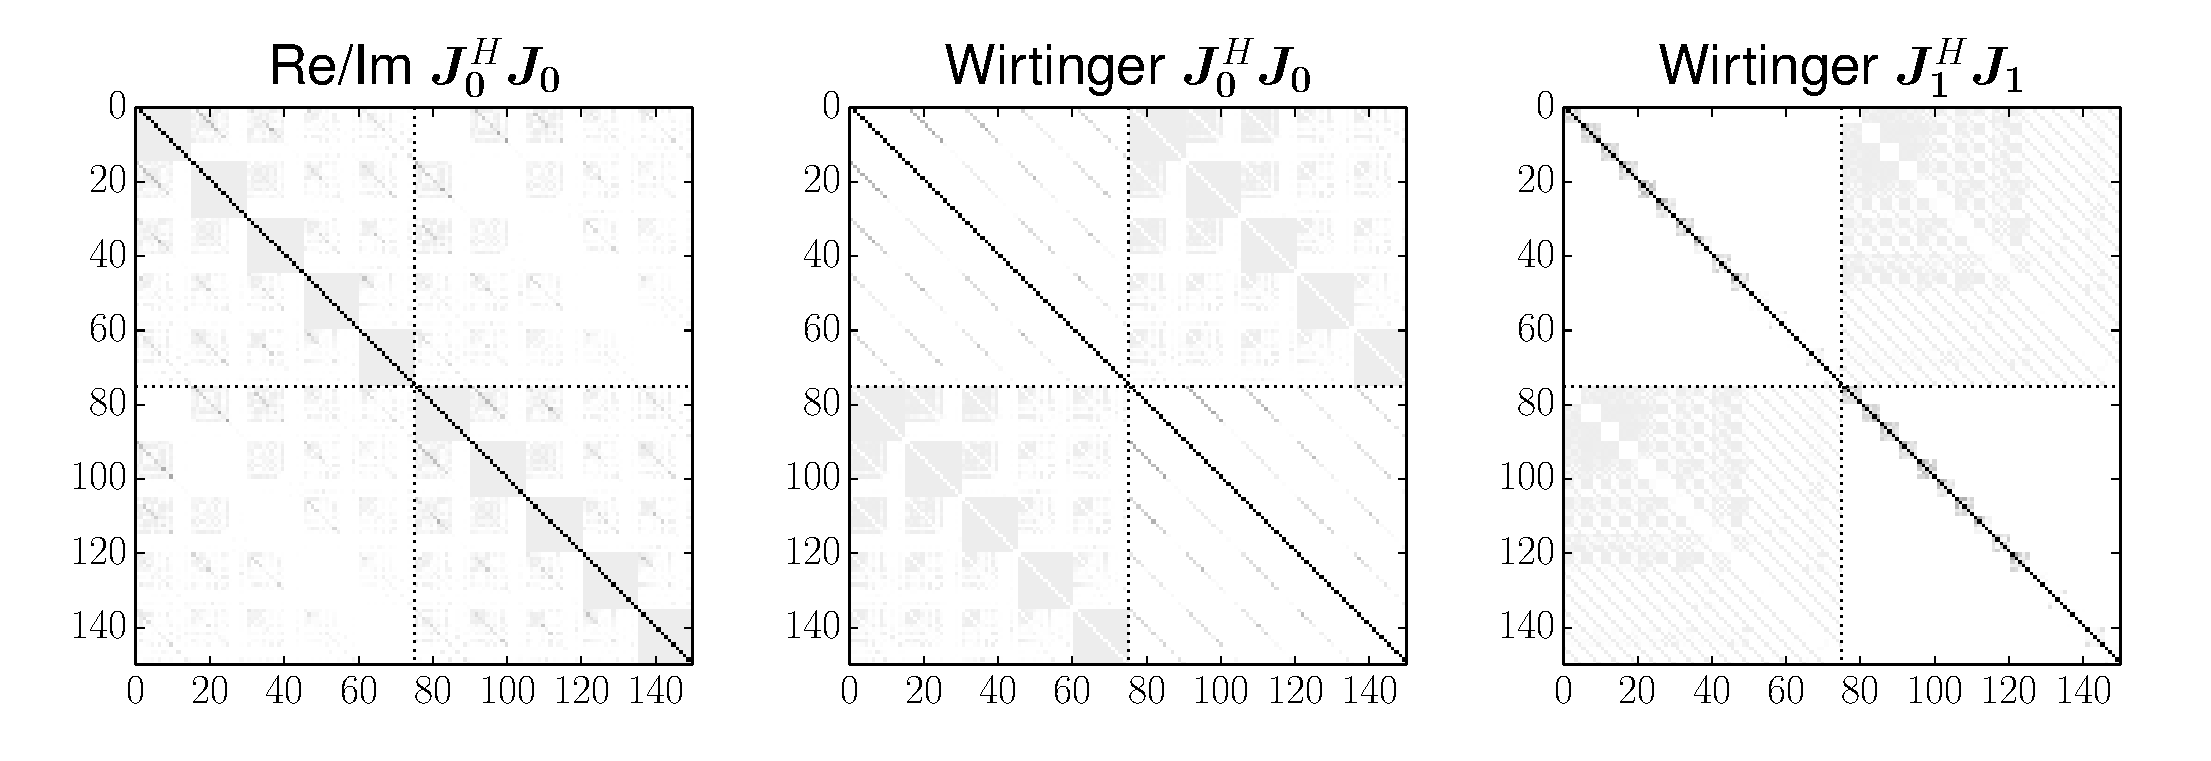
\includegraphics[width=\textwidth]{ThreeJhJ}
\caption{\label{fig:JHJ}A graphical representation of $\JHJ$ for a case of 
40 antennas and 5 directions. Each pixel represents the amplitude of a single matrix element.
(a) Conventional real-only Jacobian constructed by taking the partial
derivatives w.r.t. the real and imaginary parts of the gains; (b) full complex Jacobian where the gains 
are ordered by direction major, antenna minor; (c) full complex Jacobian where the gains are ordered by 
antenna major, direction minor. Note that (c) can also be taken to represent the direction-independent case, 
with each $5\times5$ block becoming one pixel.}
\end{center}
\end{figure*}



In this section we investigate approaches to simplifying the inversion problem by approximating
$\JJ^H\JJ$ by some form of (block-)diagonal matrix. Such approximation is equivalent to separating
the optimization problem into subsets of parameters that are treated as independent. We will show 
that some of these approximations are similar to or even fully equivalent to previously proposed 
algorithms, while others produce new algorthmic variations.

\subsection{Diagonal approximation and Stefcal}
\label{sec:DI:stefcal}

Let us first consider the DI case. The structure of $\JJ^H\JJ$ in Eq.~\ref{eq:JHJ:DI} suggests that it is diagonally 
dominant (especially for larger $\Na$), as each diagonal element is a coherent sum of $\Na$ amplitude-squared $y$-terms, 
while the off-diagonal elements are either zero or a product of two $y$ terms. This is graphically illustrated in 
Fig.~\ref{fig:JHJ}(c). It is therefore not unreasonable 
to approximate $\JHJ$ with a diagonal matrix for purposes of inversion (or equivalently, making the assumption that 
the problem is separable per antenna). This makes the costs of matrix inversion negligible -- $O(\Na)$ operations, as 
compared to the $O(\Na^2)$ cost 
of computing the diagonal elements of the Jacobian in the first place. The price of using an approximate inverse for 
$\JHJ$ is a less accurate update step, so we can expect to require more iterations before convergence is reached.

Combining this approximation with GN optimization, we may use Eq.~\ref{eq:ghat} to write out the GN update step. The diagonal
approximation consists of assuming $\bmath{B}=0$ in Eq.~\ref{eq:JHJ:DI:ABCD}. Exploiting the redundancy of the equations, we only 
need to compute the updated $\bmath{g}$ and not $\bmath{\bar g}$:

\[
\hat{\bmath{g}} = -\bmath{A}^{-1} \JJ_k^H \bmath{d},
\]

or 

\begin{equation}
\label{eq:stefcal}
\hat{g}_p = \big( \sum\limits_{q\ne p} \bar{y}_{pq} y_{pq} \big)^{-1} \sum\limits_{q\ne p} \bar{y}_{pq} d_{pq} }
\end{equation}

Note that this expression does not contain the residual term, but only the data term. This eliminates the need to 
recompute the residuals at each step (except perhaps for purposes of checking convergence). Equation~\ref{eq:stefcal} 
is identical to the update step proposed by \citet{Stefcal} for the Stefcal algorithm, and by \citet{Mitchell-RTS} for MWA calibration. Note that these authors arrive at the result from a different 
direction, by treating Eq.~\ref{eq:cal:DI} as a function of $\bmath{g}$ only, and completely ignoring the conjugate term. 
The resulting complex Jacobian (Eq.~\ref{eq:JJ:di:basic}) then has null off-diagonal blocks, and $\JJ^H\JJ$ becomes 
diagonal.

Interestingly, if apply the diagonal $\JJ^H\JJ$ approximation to LM optimization (Eq.~\ref{eq:LM1}), we can derive the following
update equation (by full analogy with Eq.~\ref{eq:GGvec}):

\[
\hat{\bmath{g}} = \frac{\lambda}{1+\lambda}\bmath{g} - \frac{1}{1+\lambda} \bmath{A}^{-1} \JJ^H \bmath{d},
\]

which for $\lambda=1$ essentially becomes the basic average-update step of Stefcal.

Establishing the equivalence between Stefcal and complex optimization with a diagonally-approximated $\JJ^H\JJ$ is 
very useful for our purposes, since the convergence properties of Stefcal have been thoroughly explored 
by \citet{Stefcal}, and we can therefore hope to apply these lessons here. In particular, these authors have shown 
that a direct application of Eq.~\ref{eq:stefcal} leads to very slow convergence, whereas averaging every pair of 
updates leads to faster convergence. They also propose a number of variations of the algorithm, all of which are 
directly applicable to the above.

Finally, let us note in passing that the update step of Eq.~\ref{eq:stefcal} is embarassingly parallel, in the sense 
that the update for each antenna is computed entirely independently.

\subsection{Separability by direction}


Now consider the problem of inverting $\JHJ$ in the DD case. This is a massive matrix, and a brute force 
approach would scale as $O(\Nd^3\Na^3)$. We can, however, adopt a few approximations. Let us first arrange the 
parameter vector in direction major, antenna minor order:

\[
\bmath{g} = [g^{(1)}_1,\dots,g^{(2)}_{N_\mathrm{ant}},g^{(2)}_1,\dots,g^{(2)}_{N_\mathrm{ant}},g^{(3)}_1,\dots ]^T
\]

The $\JHJ$ term can then be split into $\Nd\times\Nd$ blocks:

\newcommand{\JJJ}{\mathcal{J}}

\begin{equation}
\label{eq:JHJ:DD:blocked}
\JHJ = \Matrix{ccc}{\JJJ^1_1 & \dots & \JJJ^{\Nd}_1 \\
\vdots & & \vdots \\
\JJJ_{\Nd}^1 & \dots & \JJJ_{\Nd}^{\Nd} },
\end{equation}

where the structure of each $2\Na\times2\Na$ block at row $c$, column $d$, is exactly as 
given by Eq.~\ref{eq:JHJ:DD:unpol}. Figure~\ref{fig:JHJ}(b) gives a graphical representation of $\JHJ$ 
when arranged in this order.


The on-diagonal (``same-direction'') blocks $\JJJ^d_d$ will have the same structure as in the DI 
case (Eq.~\ref{eq:JHJ:DI} or Eq.~\ref{eq:JHJ:3ant}). Consider now the off-diagonal (``cross-direction'') 
blocks $\JJJ^d_c$. Their non-zero elements can take one of two forms:

\[
  \sum\limits_{q\ne i,s} \yycH_{iqs} \yyd_{iqs} = \sum\limits_{q\ne i} \ggc_q \ggdH_q \sum_s \mmcH_{iqs} \mmd_{iqs}
\]

or

\[
  \sum\limits_{s} \yyc_{jis} \yyd_{ijs} = \ggcH_i \ggdH_j \sum_s \mmcH_{ijs} \mmd_{ijs}.
\]

A common element of both is essentially a dot product of sky model components. This is a 
measure of how ``non-orthogonal'' the components are:

\begin{equation}
\label{eq:Xpqcd}
X_{pq}^{(cd)} = \left \langle \bmath{m}_{pq}^\mathrm{(c)},\bmath{m}^\mathrm{(d)}_{pq} \right \rangle = \sum_s \mmc_{pqs} \mmdH_{pqs}.
\end{equation}

We should now note that each model component will typically represent a ource of limited extent. This can be typically 
represented as

\[
\bmath{m}_{pqt\nu}^\mathrm{(d)} = S^{(d)}_{pqt\nu} k^{(d)}_{pqt\nu}, 
\]

where the term $S$ represents the visibility of that sky model component if placed phase centre. This is usually 
only weakly dependent on $t,\nu$ (in the case of a point source, for example, $S$ is just a constant flux term),
while the term

\[
k^{(d)}_{pqt,\nu} = e^{-2\pi i (\bmath{u}_{pq}(t)\cdot\bmath{\sigma}_d)\nu/c},~~~\bmath{\sigma}_d = [l_d,m_d,n_d-1]^T,
\]

represents the phase rotation to direction $\bmath{\sigma}_d$ (where $lmn$ are the corresponding direction cosines), 
given a baseline vector as a function of time $\bmath{u}_{pq}(t)$. We can then approximate the sky model dot product above as

\[
X_{pq}^{(cd)} = S^{(c)}_{pq}S^{(d)}_{pq} \sum_s e^{-2\pi i [\bmath{u}_{pq}(t)\cdot(\bmath{\sigma}_c-\bmath{\sigma}_d) ]\nu/c}
\]

The sum over samples $s$ is essentially just an integral over a complex fringe. We may expect this to be small (i.e. the
sky model components to be more orthogonal) if the directions are well-separated, and also if the sum is taken 
over longer time and frequency intervals. 

If we now assume that the sky model components are orthogonal or near-orthogonal, then 
we may treat the ``cross-direction'' blocks of the $\JHJ$ matrix in Eq.~\ref{eq:JHJ:DD:blocked} as null. The problem is 
then separable by direction, and $\JHJ$ becomes block-diagonal:


\begin{equation}
\label{eq:JHJ:DD:block-diag}
\JHJ \approx \Matrix{ccc}{\JJJ^1_1 &  & 0 \\
& \ddots &  \\
0 & & \JJJ_{\Nd}^{\Nd} },
\end{equation}


The inversion complexity then reduces to $O(\Nd)O(\Na^3)$, which, for large numbers of directions, is a huge improvement on $O(\Nd^3\Na^3)$. 

A further simplification is possible by using a Stefcal-style diagonal approximation (Sect.~\ref{sec:DI:stefcal}) for
the per-direction $\JJJ^d_d$ blocks. Matrix inversion then reduces to $O(\Nd\Na)$ in complexity, and the problem becomes dominated by
the $O(\Nd\Na^2)$ process of computing the diagonal elements of $\JHJ$. The GN update step is then a direct analogue of
Eq.~\ref{eq:update:di:unpol}:

\begin{equation}
\label{eq:update:dd:unpol}
\delta \ggd_p = \frac{\sum\limits_{q\ne p,s} \yydH_{pqs} r_{pqs}}{\sum\limits_{q\ne p,s} |\yyd_{pqs}|^2}
\end{equation}

Note, however, that unlike the DI case, where this equation directly translates into
an expression for the updated parameter vector $\hat{\bmath{g}}$ by simply replacing the residual term with the data 
term (see Eq.~\ref{eq:stefcal}), here this is no longer the case. Indeed:

\begin{equation}
\label{eq:stefcal:dd:unpol}
\begin{array}{@{}l@{}l}
\hat{g}_p^{(d)} &= \ggd_p + \frac{
\textstyle \sum\limits_{q\ne p,s} \bar{y}_{pqs} (d_{pqs} - \sum\limits_c \ggc_p \mmc_{pqs} \ggcH_q )
}{
\textstyle \sum\limits_{q\ne p,s} \bar{y}_{pqs} y_{pqs}
} \\
&= \frac{
\textstyle \sum\limits_{q\ne p,s} \bar{y}_{pqs} (d_{pqs} - \sum\limits_{c\ne d} \ggc_p \mmc_{pqs} \ggcH_q )
}{
\textstyle \sum\limits_{q\ne p,s} \bar{y}_{pqs} y_{pqs}
},
\end{array}
\end{equation}

i.e. in order to compute the updated gains vector for a particular directions $d$, the model predict towards all other 
directions $c\ne d$ must be taken into account. In practice therefore, it it probably more economical 
to use the $\delta \bmath{g}$-form (Eq.~\ref{eq:update:dd:unpol}) for updates, 
and recompute  the residuals at every iteration (though see the next section for a possible alternative). Following \citet{Stefcal}, 
we can expect to improve convergence by averaging every pair of updates together.

\subsection{Smoothing in time and frequency}
\label{sec:DI:smooth}

From physical considerations, we know that gains do not vary arbitrarily as a functions of frequency and time. It can
therefore be desirable to impose some sort of smoothness constraint on the solutions, which can improve conditioning, especially
in low-SNR situations. A simple but crude way to do this is use solution intervals (Sect.~\ref{sec:solution-intervals}),
which gives a constant gain solution per interval, but produces non-physical jumps at the edge of each interval.
Other approaches include aposteriori smoothing of solutions done on smaller intervals, as well as various filter-based 
algorithms \citep{tasse-filters}. 

Another way to impose smoothness combines the ideas of solution intervals  (Eq.~\ref{eq:cal:DI:tf}) 
and weighting (Eq.~\ref{eq:LSmin:w}). At every time/frequency sample $t_0,\nu_0$, we can postulate a weighted 
LS problem:

\begin{equation}
\label{eq:cal:DI:smooth}
\min_{\bmath{g}}\sum_{pqt\nu}w(t-t_0,\nu-\nu_0)|r_{pqt\nu}|^2, 
\end{equation}

where $w$ is a smooth weighting kernel that upweighs samples at or near the current sample, and downweighs distant 
samples (e.g., a 2D Gaussian). The solutions for adjacent samples will be very close (since they 
are constrained by practically the same range of data points, with only a smooth change in weights), and that the 
degree of smoothness can be controlled by tuning the width of the kernel.

On the face of it this approach is very expensive, since it requires that an independent LS problem be solved at 
every $t,\nu$ sample. The diagonal approximation above, however, allows for a particularly elegant and efficient way of 
implementing this in practice. Consider the weighted equations of Eqs.~\ref{eq:JHJ:DI:tfw} and \ref{eq:JHR:DI:tfw}, 
and replace the sample index $s$ by $t,\nu$. Under the diagonal approximation, the updated solution at $t_0,\nu_0$ is 
computed as:

\begin{equation}
\label{eq:stefcal:w}
\hat{g}_p(t_0,\nu_0) = \frac{\sum\limits_{q\ne p,t,\nu} w(t-t_0,\nu-\nu_0) \bar{y}_{pqt\nu} d_{pqt\nu} }
{\sum\limits_{q\ne p,t,\nu} w(t-t_0,\nu-\nu_0) \bar{y}_{pqt\nu} y_{pqt\nu}}.
\end{equation}

Looking at Eq.~\ref{eq:stefcal:w}, it's clear that both sums represent a convolution with $w$ on a discrete $t,\nu$
grid. Let us define the two functions

\[
\alpha_p(t,\nu) = \sum\limits_{q\ne p} \bar{y}_{pqt\nu} d_{pqt\nu}
\]

\[
\beta_p(t,\nu) = \sum\limits_{q\ne p} \bar{y}_{pqt\nu} y_{pqt\nu}
\]

and then an equivalent way to write Eq.~\ref{eq:stefcal:w} is

\begin{equation}
\label{eq:JHJ:diag:smooth}
\hat{g}_p(t,\nu) = \frac{w\circ \alpha_p}{w\circ\beta_p},
\end{equation}

where ``$\circ$'' represents convolution over a discrete grid.

Let's assume that $d_{pq}$ and $y_{pq}$ are loaded into memory and computed for a large chunk of $t,\nu$ values simultaneously
(any practical implementation will probably need to do this anyway, if only to take advantage of vectorized math operations on modern
CPUs and GPUs). The $\alpha_p$ and $\beta_p$ terms will then be large arrays over $t,\nu$. We can then take advantage of
the highly optimized implementations of convolution (e.g. via FFTs) that are available on most computing architectures
to implement Eq.~\ref{eq:JHJ:diag:smooth}. 

Iterating Eq.~\ref{eq:JHJ:diag:smooth} to convergence at every $t,\nu$ slot, we obtain per-antenna arrays of gain solutions 
answrering Eq.~\ref{eq:cal:DI:smooth}. These solutions are smooth in frequency and time, with the degree of smoothness 
constrained by the kernel $w$. 

\section{The Fully Polarized Case}
\label{sec:pol}

To incorporate polarization, let us start by rewriting the basic RIME of Eq.~\ref{eq:RIME:unpol} using $2\times 2$ matrices \citep[a full derivation
may be found in][]{RRIME1}:

\begin{equation}
\label{eq:RIME:pol}
\DD_{pq} = \GG_p \MM_{pq} \GG^H_q + \mat{N}_{pq}.
\end{equation}

Here, $\DD_{pq}$ is the \emph{visibility matrix} observed by baseline $pq$, $\MM_{pq}$ is the sky \emph{coherency matrix}, $\GG_p$ is the Jones matrix associated with antenna $p$, and $\mat{N}_{pq}$ is a noise matrix. Quite importantly, the visibility and coherency matrices are Hermitian: 
$\DD_{pq}=\DD^H_{qp}$, and $\MM_{pq}=\MM^H_{qp}$. The basic polarization calibration problem can be formulated as

\begin{equation}
\label{eq:cal:DI:pol}
\min_{\{\GG_p\}}\sum_{pq}||\RR_{pq}||_F,~~
\RR_{pq} = \DD_{pq}-\GG_p \MM_{pq} \GG^H_q
\end{equation}


\newcommand{\Rop}[1]{\mathcal{R}_{{#1}}}
\newcommand{\Lop}[1]{\mathcal{L}_{{#1}}}
\newcommand{\Top}{\mathcal{T}}

In principle, this can be recast into an ordinary complex NLLS problem (Eq.~\ref{eq:LSmin}) by vectorizing each 
matrix in the above equation,  and then deriving the complex Jacobian according to Eq.~\ref{eq:JJ}. We may, however, 
obtain a more elegant derivation by using a simple operator calculus, where the ``atomic'' elements are $2\times2$ matrices 
rather than scalars. We can then define the Jacobian more simply in terms of operators on such matrices. 

\subsection{Operator calculus}

First, let us introduce the vectorization operator ``vec'' and its inverse in the usual way. For a $2\times2$ matrix:

\newcommand{\VEC}[1]{\mathrm{vec}\,{#1}}
\newcommand{\VECINV}[1]{\mathrm{vec}^{-1}\,{#1}}

\[
\VEC{\mat{X}} = \Matrix{c}{x_{11}\\x_{12}\\x_{21}\\x_{22}},~~~
\VECINV{\Matrix{c}{x_{11}\\x_{12}\\x_{21}\\x_{22}}} = \mat{X},
\]

This sets up a trivial isomorphism between the space of $2\times2$ complex matrices $\COMPLEX^{2\times2}$ and the space 
$\COMPLEX^4$. Any linear operator on $\mat{X} \in \COMPLEX^{2\times2}$, which we'll write as $\mathcal{A}[\mat{X}]$, 
must then be equivalent to  multiplication of $\VEC{\mat{X}} \in \COMPLEX^4$ by some $4\times 4$ complex matrix $\mat A$. To put this formally, we can say that the $\mathrm{vec}$ operator induces an isomorphism  $\mathcal{W}$ 
between $\COMPLEX^{4\times4}$ and the space of linear 
operators on $\COMPLEX^{2\times2}$:

\begin{eqnarray}
&& \mathcal{W}:\COMPLEX^{4\times4}\leftrightarrow\mathrm{Lin}(\COMPLEX^{2\times2},\COMPLEX^{2\times2}) \nonumber\\
&& \mathcal{W}(\mat{A})[\mat{X}] = \VECINV{(\mat{A}\,\VEC{\mat{X}})} \nonumber \\
&& \mathcal{W}^{-1}(\mathcal{A})\bmath{x} = \VEC{(\mathcal{A}[ \VECINV{\bmath{x}} ])} \label{eq:iso:W}
\end{eqnarray}

Of particular interest to us are two linear operators on $\COMPLEX^{2\times2}$: right multiply by $\mat{A}$, and left multiply by $\mat{A}$, where $\mat{A}$ is a $2\times2$ complex matrix:
%, and transpose: 

\[
\begin{array}{l@{~}l}
\Rop{\mat{A}}[\mat{X}] &= \mat{XA} \\
\Lop{\mat{A}}[\mat{X}] &= \mat{AX} \\
%\Top[\mat{X}] &= \mat{X}^T
\end{array}
\]

The $\mathcal{W}$ isopmorphism ensures that these operators can be represented as multiplication of 4-vectors 
by a $4\times4$ matrix. Indeed, if $\mat{Y}=\Rop{\mat{A}}[\mat{X}]$, then 

\begin{equation}
\Matrix{c}{y_{11}\\y_{12}\\y_{21}\\y_{22}} = \VEC{\Rop{\mat{A}}[\mat{X}]} = 
\Matrix{cccc}{a_{11}&a_{21}&0&0 \\ a_{12}&a_{22}&0&0 \\ 0&0&a_{11}&a_{21} \\ 0&0&a_{12}&a_{22} }
\Matrix{c}{x_{11}\\x_{12}\\x_{21}\\x_{22}} 
\end{equation}

Likewise, 

\begin{equation}
\VEC{\Lop{\mat{A}}[\mat{X}]} = 
\Matrix{cccc}{a_{11}&0&a_{12}&0 \\ 0&a_{11}&0&a_{12} \\ a_{21}&0&a_{22}&0  \\ 0&a_{21}&0&a_{22} }
\VEC{\mat{X}}.
\end{equation}

% and

% \begin{equation}
% \VEC{\Top[\mat{X}]} = 
% \Matrix{cccc}{1&0&0&0 \\ 0&0&1&0 \\ 0&1&0&0 \\ 0&0&0&1} \VEC{\mat{X}}.
% \end{equation}

% Since $(\mat{A}\mat{X})^T = \mat{X}^T \mat{A}^T$, the superposition of a transpose and
% an $\Lop{\mat{A}}$ or $\Rop{\mat{A}}$ operator is equivalent to the opposite-hand operator using $\mat{A}^T$:

% \begin{eqnarray}
% \label{eq:LA:RATT}
% \big[ \Rop{\mat{A}^T}[\cdot] \big ]^T = \Lop{\mat{A}}[\cdot] ~~&~&~~
% \big[ \Lop{\mat{A}}[\cdot] \big]^T = \Rop{\mat{A}^T}[\cdot] \nonumber\\
% \big[ \Rop{\mat{A}^H}[\cdot] \big ]^T = \Lop{\bar{\mat{A}}}[\cdot] ~~&~&~~
% \big[ \Lop{\bar{\mat{A}}}[\cdot] \big]^T = \Rop{\mat{A}^H}[\cdot],
% \end{eqnarray}

% which we can also write as e.g.

% \begin{equation}
% \label{eq:RATT:op}
% \Lop{\mat{A}} = \Top \Rop{\mat{A}^T},~~~\Top\Lop{\mat{A}} = \Lop{\mat{A}^T}.
% \end{equation}

We may repurpose the symbols $\Rop{\mat{A}}$ and $\Lop{\mat{A}}$ to also represent the $4\times4$ matrices 
themselves. It is trivial to see that

\begin{equation}
\label{eq:RH:LH}
\Rop{\mat{A}}^H = \Rop{\mat{A}^H},~~~\Lop{\mat{A}}^H = \Lop{\mat{A}^H}.
\end{equation}

% It is easy to see that Eq.~\ref{eq:RATT:op} must necessarily hold for the $4\times4$ matrix forms as well.

% Note that the meaning of $\Top$ is specifically a transpose in $\COMPLEX^{2\times2}$ space -- it is not the same
% thing as a transpose of the $4\times4$ matrices. What $\Top$ actual does in $\COMPLEX^4$ is a swapping of vector 
% elements (i.e. swapping of rows 2 and 3). 

Other obvious properties are:

\begin{equation}
\label{eq:RAB:LAB}
\Lop{\mat{A}}\Lop{\mat{B}} = \Lop{\mat{AB}},~~~\Rop{\mat{A}}\Rop{\mat{B}} = \Rop{\mat{BA}},~~~[\Rop{\mat{A}}]^{-1} = \Rop{\mat{A^{-1}}}
\end{equation}

Note that Eq.~\ref{eq:RAB:LAB} is equally valid whether interpreted in terms of chaining operators, or multipying 
the equivalent $4\times4$ matrices.

Finally, note that the transpose and Hermitian transpose operators in $\COMPLEX^{2\times2}$ space correspond to a swapping
of the second and third rows in $\COMPLEX^4$ space:

\begin{equation}
\label{eq:vec:XH}
\VEC{\mat{X}^T} = \Matrix{c}{x_{11}\\x_{21}\\x_{12}\\x_{22}},~~~
\VEC{\mat{X}^H} = \Matrix{c}{\bar{x}_{11}\\\bar{x}_{21}\\\bar{x}_{12}\\\bar{x}_{22}}.
\end{equation}

\subsection{Derivative operators and Jacobians}

We can use the relations of Eq.~\ref{eq:iso:W} to induce a natural mapping between any matrix-valued function of a 
matrix argument $\mat{F}(\mat{G})$, $\mat{F}:\COMPLEX^{2\times2}\to\COMPLEX^{2\times2}$ and a corresponding 
vector-valued function of a vector, $\bmath{f}:\COMPLEX^4\to\COMPLEX^4$:

\[
\bmath{f}(\bmath{g}) = \VEC{\mat{F}(\VECINV{\bmath{g}})}.
\]

Consider now the partial (and conjugate partial) Jacobians of $\bmath{f}$ with respect to $\bmath{g}$ 
(and $\bar{\bmath{g}}$). These are $4\times4$ matrices (Eq.~\ref{eq:Jk}):

\[
\JJ_g = [ \partial f_i / \partial g_j ],~~~\JJ_{\bar{g}} = [ \partial f_i / \partial \bar{g}_j ]
\]

We can now use the isomorphism of Eq.~\ref{eq:iso:W} to formally define the corresponding ``Wirtinger derivative operators'' 
of $\mat{F}$ with respect to $\mat{G}$ and $\mat{G^H}$ as

\begin{equation}
\label{eq:def:dF:dG}
\frac{\partial\mat{F}}{\partial{\mat{G}}} = \mathcal{W}(\JJ_g),~~~
\frac{\partial\mat{F}}{\partial{\mat{G}^H}} = \mathcal{W}(\JJ_{\bar{g}}^T)
\end{equation}

This formal definition will allow to write the Jacobians below in terms of matrices composed of operators. 
In particular, it is easy to see (just from considering the corresponding $4\times4$ matrices) that

\[
\frac{\partial(\mat{GA})}{\partial{\mat{G}}} = \Rop{A},~~~~\frac{\partial(\mat{AG^H})}{\partial{\mat{G^H}}} = \Lop{A}.
\]

\subsection{Complex Jacobians for the polarized RIME}

Let us apply the operator calculus developed above to Eq.~\ref{eq:cal:DI:pol}. We have:

\begin{equation}
\label{eq:dR:dG}
\frac{\partial\RR_{pq}}{\partial\GG_p} = -\Rop{\MM_{pq}\GG^H_q},\mathrm{~~and~~}
\frac{\partial\RR_{pq}}{\partial\GG^H_q} = -\Lop{\GG_p \MM_{pq}}.
\end{equation}

If we now stack all the gain matrices into one ``vector of matrices'' 

\begin{equation}
\label{eq:GGvec}
\GG = [ \GG_1,\dots,\GG_{\scriptstyle \Na},\GG^H_1,\dots,\GG^H_{\scriptstyle \Na} ]^T,
\end{equation}

then we may construct the top half of the full complex Jacobian operator in full analogy with the 
derivation of Eq.~\ref{eq:JJ:di:basic}. We'll use the same ``compound index'' convention for $pq$. That is, 
$[pq]$ will represent a single index running through $M$ values (i.e. enumerating all combinations of $p<q$).

\begin{equation}
\label{eq:JJtop}
\begin{array}{r@{~}cc@{~}cc}
  & \overbrace{~~~~~~~~}^{j=1\dots \Na} & \overbrace{~~~~~~~~}^{j=1\dots \Na} \\

\JJ_\mathrm{top} = - \big [ & 
\Rop{ \MM_{pq}\GG^H_q }\delta^j_p & 
\Lop{ \GG_p \MM_{pq}  }\delta^j_q 
& \big ] ~~ \} \scriptstyle [pq]=1\dots \Nbl~(p<q)
% 
%\Lop{ \bar{\GG}_p    \bar{\MM}_{pq} }\delta^j_q & 
%\Rop{ \bar{\MM}_{pq} \bar{\GG^H_q}  }\delta^j_p  
%}.
\end{array}
\end{equation}

Note that there are two fully equivalent ways to read the above equation. In operator notation, it specifies a linear operator $\JJ_\mathrm{top}$
that maps a $2\Na$-vector of $2\times2$ matrices to an $\Nbl$-vector of $2\times2$ matrices. In conventional matrix notation, 
$\JJ_\mathrm{top}$ is just a $4\Nbl\times8\Na$ matrix; the above equation then specifies the structure of this matrix in terms
of $4\times4$ blocks, where each block is the matrix equivalent of the appropriate $\mathcal{R}$ or $\mathcal{L}$ operator.

Consider now the bottom half of the Jacobian. In Eq.~\ref{eq:JJ}, this corresponds to the derivatives of the conjugate residual
vector $\bar{\bmath{r}}_k$, and can be constructed by conjugating and mirroring $\JJ_\mathrm{top}$. Let us modify this construction 
by taking the derivative of the Hermitian transpose of the residuals. Let's construct the augmented residual vector 
as:

\begin{equation}
\bmath{R} = 
\Matrix{c}{
  \RR_{pq} \\ 
  \RR^H_{pq} 
} 
~~ 
\Stack{ 
\} \scriptstyle [pq]=1\dots \Nbl~(p<q) \\ 
\} \scriptstyle [pq]=1\dots \Nbl~(p<q) 
}
\label{eq:RRtranspose}
\end{equation}

Note that this modification is simply a matter of swapping some rows (Eq.~\ref{eq:vec:XH}) in the conjugate residual vector,
i.e. a simple change in the numbering of the residual equations. Now, since $\RR^H_{pq}=\GG_q \MM^H_{pq} \GG^H_p,$ we have

\begin{equation}
\label{eq:dRH:dG}
\frac{\partial\RR^H_{pq}}{\partial\GG_q} = -\Rop{\MM^H_{pq}\GG^H_p},\mathrm{~~and~~}
\frac{\partial\RR^H_{pq}}{\partial\GG^H_p} = -\Lop{\GG_q \MM^H_{pq}},
\end{equation}

and we may write out the complete complex Jacobian as

\[
\JJ = - \Matrix{cc}{ 
\Rop{ \MM_{pq}\GG^H_q }\delta^j_p & 
\Lop{ \GG_p \MM_{pq}  }\delta^j_q \\
\Rop{ \MM^H_{pq} \GG^H_p } \delta^j_q & 
\Lop{ \GG_q \MM^H_{pq}  } \delta^j_p  
}~~ 
\Stack{ 
\} \scriptstyle [pq]=1\dots \Nbl~(p<q) \\ 
\} \scriptstyle [pq]=1\dots \Nbl~(p<q) 
}
\]

We may now make exactly the same observation as we did to derive Eq.~\ref{eq:JJ:di}, and rewrite both $\JJ$ and $\bmath{R}$ in terms of 
a single row block. The $pq$ index will now run through $2M$ values (i.e. enumerating all combinations of $p\ne q$):

\begin{equation}
\label{eq:JJ:pol}
\JJ = - \Matrix{cc}{ 
\Rop{ \MM_{pq}\GG^H_q }\delta^j_p & 
\Lop{ \GG_p \MM_{pq}  }\delta^j_q \\
}~~ 
\} \scriptstyle [pq]=1\dots 2\Nbl~(p\ne q)\\ 
\end{equation}

and 

\begin{equation}
\bmath{r} = \Matrix{c}{ \mat{R}_{pq}}~~ 
\} \scriptstyle [pq]=1\dots 2\Nbl~(p\ne q)\\ 
\end{equation}

This is in complete analogy to the derivations of the unpolarized case. For compactness, let us now define

\newcommand{\YY}{\mat{Y}}
\newcommand{\ZZ}{\mat{Z}}
\[
\YY_{pq} = \MM_{pq} \GG^H_q,
\]

and, noting that 

\[
\YY_{qp}^H = \GG_p \MM_{pq},
\]

and using Eq.~\ref{eq:RH:LH}, we can now write out the $\JHJ$ term, still expressed in terms of 
operators, as:
%\footnote{The Hermitian conjugate operators are derived as $\Rop{\mat{A}}^H=\Rop{\mat{A}^H}$ and 
%$\Lop{\mat{A}}^H=\Lop{\mat{A}^H}$, see Appendix~\ref{sec:4x4app}.} 

\begin{equation}
\label{eq:JHJ:pol}
\JHJ = \JHJblocks{
  \mathrm{diag}\sum\limits_{q\ne i} \Rop{\YY_{iq} \YY^H_{iq}} 
}{
% & 
%   \left \{ 
%   \begin{array}{@{}cc@{}}
%    \Rop{ \YY^H_{ij}  } \Lop{\YY^H_{ji}},&{\scriptstyle i\ne j} \\
%    0, &{\scriptstyle i=j}
%   \end{array} \right . 
%   \\
  \left \{ 
  \begin{array}{@{}cc@{}}
   \Lop{ Y_{ji}  } \Rop{\YY_{ij}},&{\scriptstyle i\ne j} \\
   0, &{\scriptstyle i=j}
  \end{array} \right . 
}
  % &
  % \mathrm{diag}\sum\limits_{q\ne i} \Lop{\YY^H_{qi}\YY_{qi}}
\end{equation}

(Note that this makes use of the property $\Rop{\mat{A}}\Rop{\mat{B}}=\Rop{\mat{BA}}$ and 
$\Lop{\mat{A}}\Lop{\mat{B}}=\Lop{\mat{AB}}$.) Compare this result to Eq.~\ref{eq:JHJ:DI}.

For the $\JJ^H\bmath{R}$ term, we can directly apply the linear operators appearing in $\JJ^H$ 
to the matrices in $\bmath{R}$:

\begin{equation}
\JJ^H\bmath{R} = -\Matrix{c}{ 
\sum\limits_{pq} \YY^H_{pq} \RR_{pq} \delta^{i}_p  \\
\hline\\[-8pt]
\sum\limits_{pq} \RR_{pq} \YY_{qp} \delta^{i}_q 
} = -\Matrix{c}{
\sum\limits_{q\ne i} \YY^H_{iq} \RR_{iq} \\
\hline\\[-8pt]
\downarrow^H
%\sum\limits_{q\ne i} \RR^H_{iq} \YY_{iq}  
},
% \Stack{ 
% \big \} \scriptstyle i=1\dots \Na \\ 
% \big \} \scriptstyle i=1\dots \Na,
% }
\end{equation}

where the second equality is established by swapping the $p$ and $q$ indices. Unsurprisingly, and by analogy with 
Eq.~\ref{eq:JHR:DI1}, the bottom half of the vector is Hermitian with respect to the top.

To actually implement GN or LM optimization, we still need to invert the matrix represented (in operator form) 
by Eq.~\ref{eq:JHJ:pol}. We have two options here. The brute-force numerical approach is to substitute the 
$4\times4$ matrix forms of $\Rop{~}$ and $\Lop{~}$ into the equation, thus resulting in conventional matrix,
and then do a straightfoward matrix inversion. The second option is to use an analogue of the diagonal 
approximation described in Sect.~\ref{sec:DI:stefcal}. If we neglect the off-diagonal operators of Eq.~\ref{eq:JHJ:pol}, 
the operator form of the matrix is diagonal, and the problem is separable per antenna. The inverse operator 
corresponding to $\Rop{\mat{A}}$ is, trivially, $\Rop{\mat{A}^{-1}}$. We then arrive a simple per-antenna equation 
for the GN update step:

\begin{equation}
\label{eq:update:DI:diag:pol}
\hat{\GG}_p = \left [ \sum\limits_{q\ne p} \YY^H_{pq} \DD_{pq} \right ] 
\left [ \sum\limits_{q\ne p} \YY_{pq} \YY^H_{pq}  \right ]^{-1}
\end{equation}

This is once again equivalent to the polarized Stefcal update step proposed by \citet{Stefcal}. 
% Note also that all 
% the tricks of weighting and time/frequency averaging or smoothing discussed in Sect.~\ref{sec:DI:W}--\ref{sec:DI:smooth} 
% can also be applied in this formulation.


\subsection{Polarized direction-dependent calibration}

Let us now briefly address the fully-polarized DD case. This can be now done by direct analogy with
Sect.~\ref{sec:unpol:DD}, using the operator calculus developed above. As a result, we arrive at the
following expression for $\JHJ$:

\begin{equation}
\label{eq:JHJ:DD:pol}
  \JHJ = \JHJblocks{
  \delta^i_j \sum\limits_{q\ne i,s} \Rop{\YYd_{iqs} \YYcH_{iqs}} 
  % & 
  % \left \{ 
  % \begin{array}{@{}cc@{}}
  %  \sum\limits_{s} \Rop{ \YYcH_{ijs}  } \Lop{\YYdH_{jis}},&{\scriptstyle i\ne j} \\
  %  0 &{\scriptstyle i=j}
  % \end{array} \right . 
  % \\
  }{
  \left \{ 
  \begin{array}{@{}cc@{}}
   \sum\limits_{s} \Lop{ \YYc_{jis}  } \Rop{\YYd_{ijs}},&{\scriptstyle i\ne j} \\
   0 &{\scriptstyle i=j}
  \end{array} \right . 
  }
  % &
  % \delta^i_j \sum\limits_{q\ne i,s} \Lop{\YYcH_{qis}\YYd_{qis}}
,
\end{equation}

using the normal shorthand of $\YYd_{pqs} = \MMd_{pqs} \GGdH_q$. The $\JJ^H\bmath{R}$ term is then

\newcommand{\CCC}{\mathcal{C}}

\begin{equation}
\label{eq:JHR:DD:pol}
\JJ^H\bmath{R} = -\Matrix{c}{
\sum\limits_{q\ne i,s} \YYdH_{iqs} \RR_{iqs} \\
\hline\\[-8pt]
\downarrow^H}.
%\sum\limits_{q\ne i,s} \RR^H_{iqs} \YYd_{iqs}  } 
\end{equation}

Using both the direction separability and antenna separability assumptions above, the GN update step can be computed as

\begin{equation}
\label{eq:update:DD:diag:pol}
\delta \GGd_p = \left [ \sum\limits_{q\ne p,s} \YYdH_{pqs} \RR_{pqs} \right ] 
\left [ \sum\limits_{q\ne p,s} \YYd_{pqs} \YYdH_{pqs}  \right ]^{-1}
\end{equation}

Note that it is straightfoward to add weights and/or sliding window averging to this formulation, as per 
Sect.~\ref{sec:DI:W} and \ref{sec:DI:smooth}.

Equations~\ref{eq:JHJ:DD:pol}--\ref{eq:JHR:DD:pol} can be considered the principal result of this work.
They provide the necessary ingredients for implementing GN or LM methods for DD calibration, treating it as a 
fully complex optimization problem. As we'll show below, the equations may be combined and approximated in different 
ways to produce different types of calibration algorithms. In particular, under both separability assumptions, we can 
apply GN to derive what is essentially a generalization of Stefcal to DD solutions. An application of this algorithm to 
real data is presented in Sect.~\ref{sec:realdata}.

Another interesting note is that Eq.~\ref{eq:update:DD:diag:pol} is embarassingly parallel, since the update step is 
completely separated by direction and antenna. This makes it particularly well-suited to implementation on massively 
parallel architectures such as GPUs.

\section{Other algorithmic variations}

The mathematical framework developed above (in particular, Eqs.~\ref{eq:JHJ:DD:pol}--\ref{eq:JHR:DD:pol}) provides
a general description of the polarized DD calibration problem. Practical implementations of this hinge around inversion of
a very large $\JHJ$ matrix. In this context, we can view ``DD-Stefcal'' (Eq.~\ref{eq:update:DD:diag:pol}) as just one 
possible approximation to the inversion problem. The convergence properties of 
DD-Stefcal are not yet well-understood; established properties of DI-Stefcal \citep{Stefcal} are encouraging, but ought not 
be treated as anything more than a strong pointer for the DD case. It is therefore well worth exploring other approximations to 
the problem. In this section we map out a few such options.

\subsection{Feed forward}
\label{sec:feed-forward}

\citet{Stefcal} propose variants of the Stefcal algorithm (``2-basic'' and ``2-relax'') where the results of the 
update step (Eq.~\ref{eq:update:DI:diag:pol}, in essense) are computed sequentially per antenna, with updated
values for $\GG_1,\dots,\GG_{k-1}$ fed forward into the equations for $\GG_k$. This is shown to 
substantially improve convergence, at the cost of sacrificing the embarassing paralellism by antenna. This technique 
is directly applicable to Eq.~\ref{eq:update:DD:diag:pol}. 

An interesting variation to explore is feed forward by direction. In Eq.~\ref{eq:update:DD:diag:pol}, the DD gain 
update is computed independently for each direction (since one of the approximations made is that the ``cross-direction''
blocks $\JJJ^c_d$ are null). From practical experience, we know that inaccuracies towards brighter 
sources will tend to affect solutions towards fainter sources. We can therefore expect to improve convergence
by incorporating information about DD gains towards brighter sources in the solutions for the fainter ones. There are
a few approaches to this. One is a direct extension of the feed forward idea. Assuming 
the sky model components are ordered by decreasing brightness (and revisiting Eq.~\ref{eq:update:dd:unpol}), we may:

\begin{enumerate}
\item Compute the direction-1 residuals, by subtracting every sky model component except the first:
\[
  \RR^{(1)}_{pqs} = \DD_{pqs} - \sum\limits_{d\ne1} \GGd_p \MMd_{pqs} \GGdH_q .
\]
\item Compute an update for direction 1, all antennas: $\GG^{(1)}_1,\dots,\GG^{(1)}_{\Na}$ (optionally using feed forward
for the antenna solutions):

\[
\hat{\GG}^{(1)}_p = \left [ \sum\limits_{q\ne p,s} \YYdH_{pqs} \RR^{(1)}_{pqs} \right ] 
\left [ \sum\limits_{q\ne p,s} \YYd_{pqs} \YYdH_{pqs}  \right ]^{-1}
\]

\item Compute the direction-2 residuals as
\[
  \RR^{(2)}_{pqs} = \RR^{(1)}_{pqs} - \hat{\GG}^{(1)}_p \MM^{(1)}_{pqs} \hat{\GG}^{(1)H}_q + \GG^{(2)}_p \MM^{(2)}_{pqs} \GG^{(2)H}_q
\]

\item Go to step (ii) to compute $\hat{\GG}^{(2)}_p$, etc.

\end{enumerate}

Intuitively, this procedure corresponds to feeding the estimates obtained for directions $1,...,k-1$ forward into the 
equations for direction $k$. Whether in practice this actually improves convergence to justify the extra complexity remains to be seen.

\subsection{Triangular approximation}

Another approach to incorporating directions $1,...,k-1$ into the solution for $k$ is to approximate the $\JHJ$ matrix as
block-triangular:

\begin{equation}
\label{eq:JHJ:DD:block-triag}
\JHJ \approx \Matrix{cccc}{
\JJJ^1_1 & 0 & \cdots & 0 \\
\JJJ^1_2 & \JJJ^2_2 & \cdots & 0 \\
\vdots & & \ddots &  \vdots \\
\JJJ_{\Nd}^1 & \JJJ_{\Nd}^2 & \cdots & \JJJ_{\Nd}^{\Nd} },
\end{equation}

\newcommand{\KKK}{\mathcal{K}}

The inverse of this is also block triangular:
\begin{equation}
\label{eq:JHJ:DD:block-triag-inv}
\KKK = \JHJ^{-1} = \Matrix{cccc}{
\KKK^1_1 & 0 & \cdots & 0 \\
\KKK^1_2 & \KKK^2_2 & \cdots & 0 \\
\vdots & & \ddots &  \vdots \\
\KKK_{\Nd}^1 & \KKK_{\Nd}^2 & \cdots & \KKK_{\Nd}^{\Nd} },
\end{equation}
which can be computed using Gaussian elimination:

\[
\begin{array}{l@{~}l}
\KKK^1_1 &= [\JJJ^1_1]^{-1} \\
\KKK^2_2 &= [\JJJ^2_2]^{-1} \\
\KKK^1_2 &= - \KKK^2_2 \JJJ^1_2 \KKK^1_1\\
\KKK^3_3 &= [\JJJ^3_3]^{-1} \\
\KKK^2_3 &= - \KKK^3_3 \JJJ^2_3 \KKK^2_2\\
\KKK^1_3 &= - \KKK^3_3 [ \JJJ^1_3 \KKK^1_1 + \JJJ^2_3 \KKK^1_2  ]\\
\cdots
\end{array}
\]

The GN update equations then take the following form (not forgetting $\KKK$ is in operator notation):

\[
\delta \GG^{(d)}_p = \sum\limits_{c=1}^d \KKK^c_d \left [ \sum\limits_{q\ne p,s} \YY^{(c)H}_{pqs} \RR_{pqs}  \right ],
\]

i.e. the update for direction $d$ explictly incorporates information on directions $1,...,d-1$. The corresponding matrix operations 
are cumbersome to write out, but are straightforward to implement algorithmically.



% Let's again assume the diagonal approximation for inverting the $\JJJ^c_d$ blocks (recalling -- see Eq.~\ref{eq:JHJ:pol} -- that
% $\JJJ$ and $\KKK$ are in operator notation, and correspond to matrix multiplication \emph{from the right}). Let's also define
% two shorthands:

% \[
% \mat{C}^{(d)}_p = \sum\limits_{q\ne p,s} \YY^{(d)H}_{pqs} \RR_{pqs},~~
% \mat{K}^{(cd)}_p = \sum\limits_{q\ne p,s} \YY^{(d)}_{pqs} \YY^{(c)H}_{pqs},
% \]

% so that the standard GN update equations (Eq.~\ref{eq:update:DD:diag:pol}) are simply $\delta \GGd_p = \mat{C}^{(d)}_p \mat{K}^{(dd)-1}_p$.

% For example,

% \[
% \begin{array}{l@{~}l}
% \delta \GG^{(1)}_p &= \mat{C}^{(1)}_p \mat{K}^{(11)-1}_p \\
% \delta \GG^{(2)}_p &= [ \mat{C}^{(2)}_p - \delta \GG^{(1)}_p \mat{K}^{(21)}_p ] \mat{K}^{(22)-1}_p 
% \end{array}
% \]

\subsection{Peeling}
\label{sec:peeling}

The \emph{peeling} procedure was originally suggested by \citet{JEN:peeling} as a ``kludge'', i.e. an implementation of DD calibration 
using the DI functionality of existing packages. In a nutshell, this procedure solves for DD gains towards one source at a time, from
brighter to fainter, by

\begin{enumerate}
\item Rephasing the visibilities to place the source at phase centre;
\item Averaging over some time/frequency interval (to suppress the contribution of other sources);
\item Doing a standard solution for DI gains (which approximates the DD gains towards the source);
\item Subtracting the source from the visibilities using the obtained solutions;
\item Repeating the procedure for the next source.
\end{enumerate}

The term ``peeling'' comes from step (iv), since sources are ``peeled'' away one at a time\footnote{The term ``peeling'' has 
occasionally been misappropriated to describe other schemes, e.g. simultaneous independent DD gain solutions. We consider this a 
misuse: both the original formulation by \citet{JEN:peeling}, and the word ``peeling'' itself, strongly implies dealing with 
one direction at a time.}.

Within the framework above, peeling can be considered as the ultimate feed forward approach. Peeling is essentially similar to 
the procedure in Sect.~\ref{sec:feed-forward}, except rather than taking just one step, each direction is iterated to full 
convergence before moving on to the next direction. The procedure can then be repeated beginning with the brightest source again,
a second cycle tends to improve the solutions. 

\subsection{Semi-exact Gauss-Newton and Levenberg-Marquardt}

In the authors' experience \citep{OMS-Stefcal}, an LM implementation of the DI calibration problem converges in fewer steps 
than Stefcal, but is almost always slower in terms of ``wall time'' due to the more expensive iterations. This is a 
typical ``cheap--approximate'' versus ``expensive--accurate'' trade-off, consistent with the expected scaling properties 
of the algorithms. It is the diagonal (separable by antenna) approximation that makes for cheap matrix inversion.

However, with low $\Na$ there may still be regimes where approaches with slower yet more precise update steps may have an advantage. 
It is therefore worth noting how these can fit within our framework. 

Recall again that in the direction-dependent case there are two approximations that keep the inversion of $\JHJ$ (an $O(\Nd^3\Na^3)$ problem if brute-forced) tractable:

\begin{itemize}
\item We separate the problem by direction, approximating $\JHJ$ as block-diagonal (Eq.~\ref{eq:JHJ:DD:block-diag}) or block-triangular
(Eq.~\ref{eq:JHJ:DD:block-triag}).
\item We separate the problem by antenna, approximating each block $\JJJ^d_d$ as diagonal or $2\times2$ block-diagonal. 
\end{itemize} 

We can avoid the second approximation, and compute the true inverse of each $\JJJ^d_d$. The problem then becomes
$O(\Nd\Na^3)$ in complexity, but the update steps are presumably more precise, and the LM method may be applied as well. Whether
this offers any performance advantage (again, conceivably only in a low-$\Na$ regime) remains to be seen.

The complementary alternative is to avoid the first approximation instead, and rearrange the rows of the Jacobian so that $\JHJ$ 
can be decomposed into blocks by antenna, each of size $\Nd\times\Nd$:

\newcommand{\JJX}{\tilde{\JJJ}}
\begin{equation}
\label{eq:JHJ:DD:blocked-ant}
\JHJ = \Matrix{ccc}{\JJX^1_1 & \dots & \JJX^{\Na}_1 \\
\vdots & & \vdots \\
\JJX_{\Na}^1 & \dots & \JJX_{\Na}^{\Na} }.
\end{equation}

If we then assume the problem is separable by antenna, then we ignore the cross-antenna blocks $\JJX^p_q$, and treat this 
matrix as block-diagonal, computing the true inverse of each $\JJX^p_p$. The problem then reduces to $O(\Nd^3\Na)$ in complexity, 
and LM again becomes an option. This approach has not been tested, but it could perhaps offer some performance advantages in a low-$\Nd$ regime.



\section{Implementation and real data}

\subsection{Stefcal in MeqTrees}

Some of the ideas above have already been implemented in the MeqTrees \citep{meqtrees} version of Stefcal 
\citep{OMS-Stefcal}. In particular, the MeqTrees version uses peeling (Sect.~\ref{sec:peeling}) to deal with
DD solutions, and implements polarized Stefcal with support for both solution intervals and time/frequency smoothing 
with a Gaussian kernel (as per Sect.~\ref{sec:DI:smooth}). This has already been applied to JVLA L-band data 
to obtain what is (at time of writing) a world record dynamic range (3.2 million) image of the field 
around 3C147 \citep{Perley-3C147}.

\subsection{DD-Stefcal}



\begin{figure*}
\begin{center}
%\hspace*{-1.3cm}
\includegraphics[width=\textwidth]{resid}
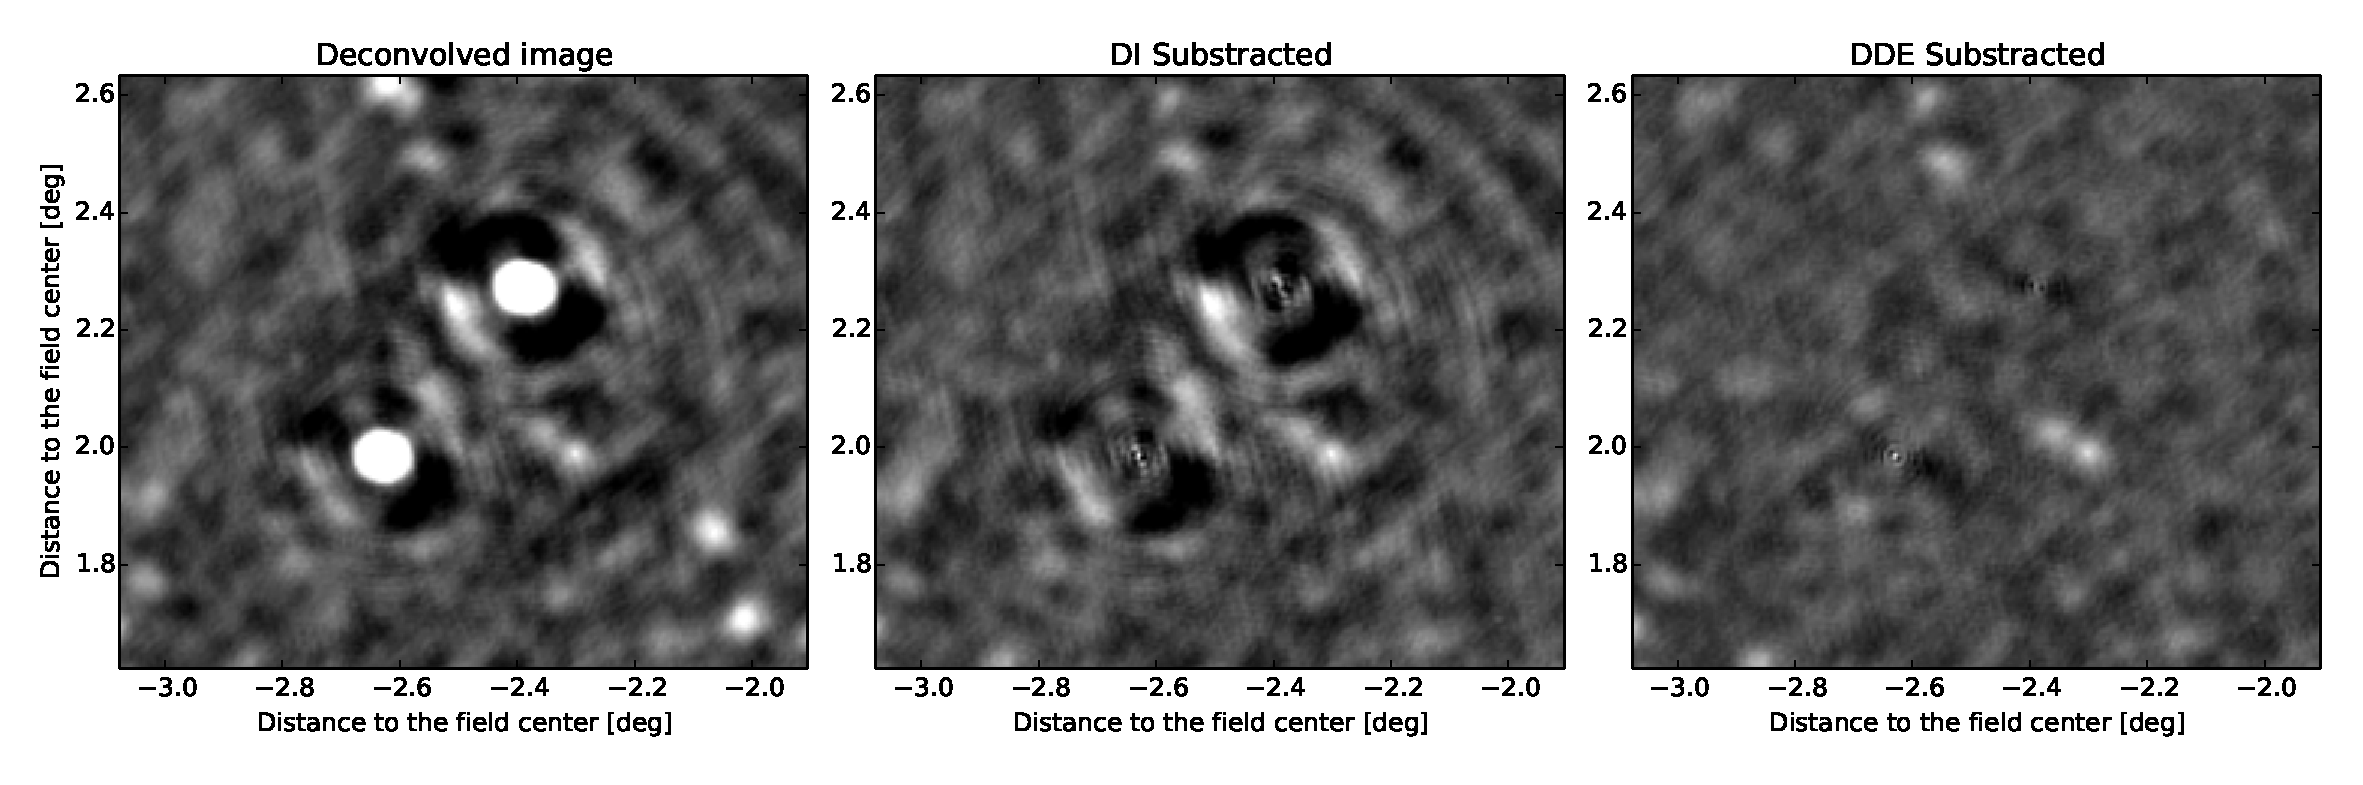
\includegraphics[width=\textwidth]{residZoom}
\caption{\label{fig:resid} This figure shows compares the image
  (left), the residuals data after simple skymodel substraction
  (center), and the residuals data after substracting the
  sky model corrupted by the direction-dependent solution (right).}
\end{center}
\end{figure*}


We test the ``DD-Stefcal'' variation described above (Eq.~\ref{eq:update:DD:diag:pol}) on a LOFAR observation of 3C295. The
visibilities produced by this interferometer are predominantly affected by direction dependent effects including (i) the 
phased beam instability and deviation from the
theoritical model, (ii) ionosphere time delays shifts, and (iii) Faraday rotation.

We first calibrate the dataset using BBS, and in order to build a pertinent model of the field, we substract 3C295. We extract the
sources using pyBDSM. The sources are the clustered in 10 directions using Voronoitesselation (fig. \ref{fig:tessel}). In Fig.~\ref{fig:resid}, we compare the residuals as
computed by substracting the model data in the visibility domain, and the model data affected by DDEs.




\begin{figure}[]
\begin{center}
%\hspace*{-1.3cm}
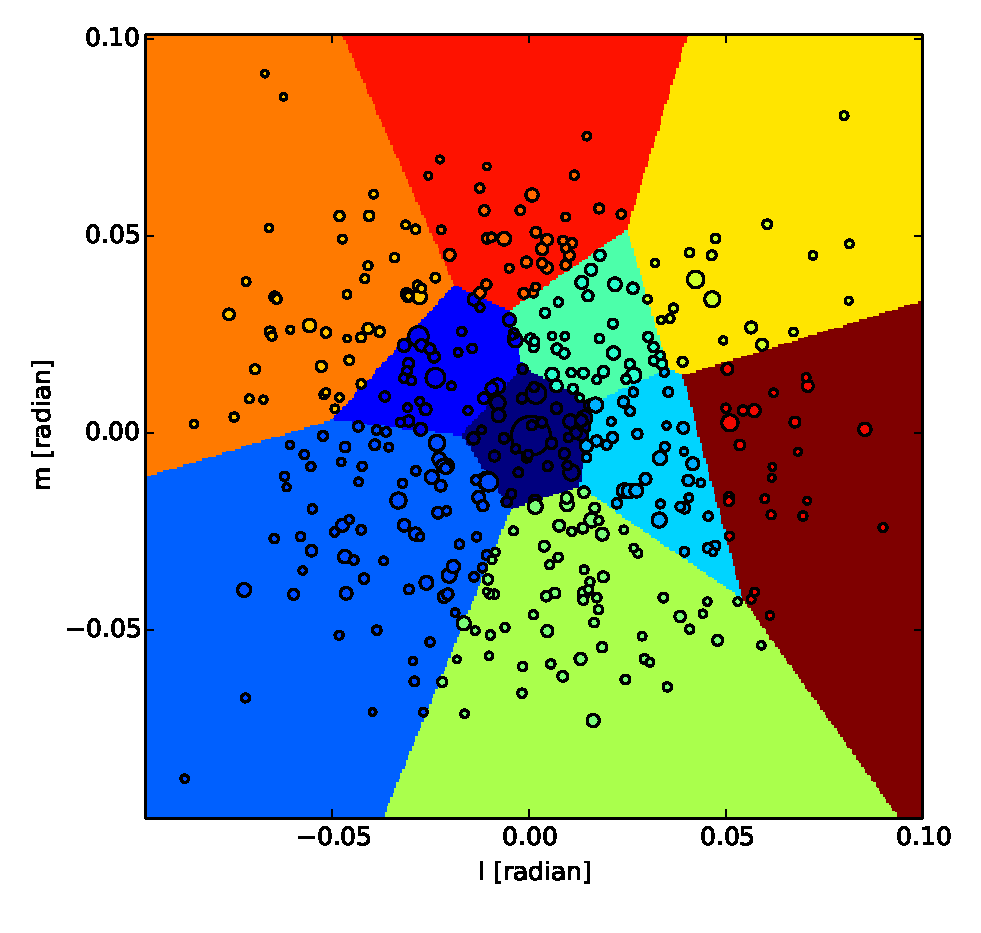
\includegraphics[width=\columnwidth]{tessel}
\caption{\label{fig:tessel} In order to minimize the number of degrees
of freedom, and increase the amount of signal in each direction, we cluster the sources in 10 direction using a Voronoi
tesselation.}
\end{center}
\end{figure}



\label{sec:realdata}

\section*{Conclusions}

Complexity $O(\mathrm{chicken}).$ Chicken!

Embarassingly parallel. GPU. Chicken!

Many variations possible, describes previous algorithms as special cases (approximations). Chicken!

Unifying framework? Chicken!

\bibliographystyle{mn2e}
\bibliography{cjpaper}

\appendix

\section{$\JJ$ and $\JJ^H\JJ$ for the three-antenna case}
\label{sec:3ant}

To give a specific example of complex Jacobians, consider the 3 antenna case.
Using the numbering convention for $pq$ of 12, 13, 32, we obtain the following partial Jacobians
(Eqs.~\ref{eq:Jk} and \ref{eq:Jbark}):

\[
\JJ_k = - \Matrix{ccc}{m_{12}\bar{g}_2 & 0 & 0 \\ m_{13}\bar{g}_3 & 0 & 0 \\ 0 & m_{23}\bar{g}_3 & 0 },
\JJ_{\bar{k}} = - \Matrix{ccc}{0 & g_1 m_{12} & 0 \\ 0 & 0 & g_1 m_{13} \\ 0 & 0 & g_2 m_{23} }
\]

We then get the following expression
for the full complex Jacobian $\JJ$ (Eq.~\ref{eq:JJ:di}):

\begin{equation}
\label{eq:JJ:3ant}
-\Matrix{cccccc}{
  m_{12}\bar{g}_2 & 0               & 0 &  0          & g_1 m_{12} & 0           \\
  m_{13}\bar{g}_3 & 0               & 0 &  0          & 0          & g_1 m_{13}  \\
  0               & m_{21}\bar{g}_1 & 0 &  g_2 m_{21} & 0          & 0  \\
  0               & m_{23}\bar{g}_3 & 0 &  0          & 0          & g_2 m_{23} \\
  0               & 0               & m_{31}\bar{g}_1 & g_1 m_{31} & 0          & 0  \\
  0               & 0               & m_{32}\bar{g}_2 & 0 & g_3 m_{32} & 0 \\
}
\end{equation}



Then, with the usual shorthand of $y_{pq} = m_{pq} \bar{g}_q$, the
$\JJ^H\JJ$ term becomes:

\begin{equation}
\label{eq:JHJ:3ant}
\Matrix{@{~}c@{}c@{}c@{}c@{}c@{}c@{~}}{
\scriptstyle\yysq{12}{13} &\scriptstyle 0             &\scriptstyle 0             &\scriptstyle 0             &\scriptstyle \bb{1}{2}       &\scriptstyle \bb{1}{3} \\
\scriptstyle0             &\scriptstyle \yysq{12}{23} &\scriptstyle 0             &\scriptstyle \bb{1}{2}       &\scriptstyle 0             &\scriptstyle \bb{2}{3} \\
\scriptstyle0             &\scriptstyle 0             &\scriptstyle \yysq{13}{23} &\scriptstyle \bb{1}{3}       &\scriptstyle \bb{2}{3}       &\scriptstyle 0       \\
\scriptstyle0             &\scriptstyle \bbb{1}{2}      &\scriptstyle \bbb{1}{3}      &\scriptstyle \yysq{12}{13} &\scriptstyle 0             &\scriptstyle 0       \\ 
\scriptstyle\bbb{1}{2}      &\scriptstyle 0             &\scriptstyle \bbb{2}{3}      &\scriptstyle 0             &\scriptstyle \yysq{12}{23} &\scriptstyle 0 \\
\scriptstyle\bbb{1}{3}      &\scriptstyle \bbb{2}{3}      &\scriptstyle 0             &\scriptstyle 0             &\scriptstyle 0             &\scriptstyle  \yysq{13}{23} \\
}
\end{equation}

Finally, the 3-antenna $\JJ^H\bmath{r}$ term becomes

\begin{equation}
\label{eq:JHR:3ant}
\JJ^H\bmath{r} = \Matrix{c}{
\bar{y}_{12} r_{12} + \bar{y}_{13} r_{13} \\
\bar{y}_{21} r_{21} + \bar{y}_{23} r_{23} \\
\bar{y}_{31} r_{31} + \bar{y}_{32} r_{32} \\
y_{12} \bar{r}_{12} + y_{13} \bar{r}_{13}   \\
y_{21} \bar{r}_{21} + y_{23} \bar{r}_{23}   \\
y_{31} \bar{r}_{31} + y_{32} \bar{r}_{32}   \\
}.
\end{equation}




\label{lastpage}

\end{document}